% Options for packages loaded elsewhere
\PassOptionsToPackage{unicode}{hyperref}
\PassOptionsToPackage{hyphens}{url}
\PassOptionsToPackage{dvipsnames,svgnames,x11names}{xcolor}
%
\documentclass[
  article,
  nofooter,
  noheadings]{jss}

\usepackage{amsmath,amssymb}
\usepackage{iftex}
\ifPDFTeX
  \usepackage[T1]{fontenc}
  \usepackage[utf8]{inputenc}
  \usepackage{textcomp} % provide euro and other symbols
\else % if luatex or xetex
  \usepackage{unicode-math}
  \defaultfontfeatures{Scale=MatchLowercase}
  \defaultfontfeatures[\rmfamily]{Ligatures=TeX,Scale=1}
\fi
\usepackage{lmodern}
\ifPDFTeX\else  
    % xetex/luatex font selection
\fi
% Use upquote if available, for straight quotes in verbatim environments
\IfFileExists{upquote.sty}{\usepackage{upquote}}{}
\IfFileExists{microtype.sty}{% use microtype if available
  \usepackage[]{microtype}
  \UseMicrotypeSet[protrusion]{basicmath} % disable protrusion for tt fonts
}{}
\makeatletter
\@ifundefined{KOMAClassName}{% if non-KOMA class
  \IfFileExists{parskip.sty}{%
    \usepackage{parskip}
  }{% else
    \setlength{\parindent}{0pt}
    \setlength{\parskip}{6pt plus 2pt minus 1pt}}
}{% if KOMA class
  \KOMAoptions{parskip=half}}
\makeatother
\usepackage{xcolor}
\setlength{\emergencystretch}{3em} % prevent overfull lines
\setcounter{secnumdepth}{-\maxdimen} % remove section numbering
% Make \paragraph and \subparagraph free-standing
\makeatletter
\ifx\paragraph\undefined\else
  \let\oldparagraph\paragraph
  \renewcommand{\paragraph}{
    \@ifstar
      \xxxParagraphStar
      \xxxParagraphNoStar
  }
  \newcommand{\xxxParagraphStar}[1]{\oldparagraph*{#1}\mbox{}}
  \newcommand{\xxxParagraphNoStar}[1]{\oldparagraph{#1}\mbox{}}
\fi
\ifx\subparagraph\undefined\else
  \let\oldsubparagraph\subparagraph
  \renewcommand{\subparagraph}{
    \@ifstar
      \xxxSubParagraphStar
      \xxxSubParagraphNoStar
  }
  \newcommand{\xxxSubParagraphStar}[1]{\oldsubparagraph*{#1}\mbox{}}
  \newcommand{\xxxSubParagraphNoStar}[1]{\oldsubparagraph{#1}\mbox{}}
\fi
\makeatother


\providecommand{\tightlist}{%
  \setlength{\itemsep}{0pt}\setlength{\parskip}{0pt}}\usepackage{longtable,booktabs,array}
\usepackage{calc} % for calculating minipage widths
% Correct order of tables after \paragraph or \subparagraph
\usepackage{etoolbox}
\makeatletter
\patchcmd\longtable{\par}{\if@noskipsec\mbox{}\fi\par}{}{}
\makeatother
% Allow footnotes in longtable head/foot
\IfFileExists{footnotehyper.sty}{\usepackage{footnotehyper}}{\usepackage{footnote}}
\makesavenoteenv{longtable}
\usepackage{graphicx}
\makeatletter
\newsavebox\pandoc@box
\newcommand*\pandocbounded[1]{% scales image to fit in text height/width
  \sbox\pandoc@box{#1}%
  \Gscale@div\@tempa{\textheight}{\dimexpr\ht\pandoc@box+\dp\pandoc@box\relax}%
  \Gscale@div\@tempb{\linewidth}{\wd\pandoc@box}%
  \ifdim\@tempb\p@<\@tempa\p@\let\@tempa\@tempb\fi% select the smaller of both
  \ifdim\@tempa\p@<\p@\scalebox{\@tempa}{\usebox\pandoc@box}%
  \else\usebox{\pandoc@box}%
  \fi%
}
% Set default figure placement to htbp
\def\fps@figure{htbp}
\makeatother

\usepackage{orcidlink,thumbpdf,lmodern}

\newcommand{\class}[1]{`\code{#1}'}
\newcommand{\fct}[1]{\code{#1()}}
\makeatletter
\@ifpackageloaded{tcolorbox}{}{\usepackage[skins,breakable]{tcolorbox}}
\@ifpackageloaded{fontawesome5}{}{\usepackage{fontawesome5}}
\definecolor{quarto-callout-color}{HTML}{909090}
\definecolor{quarto-callout-note-color}{HTML}{0758E5}
\definecolor{quarto-callout-important-color}{HTML}{CC1914}
\definecolor{quarto-callout-warning-color}{HTML}{EB9113}
\definecolor{quarto-callout-tip-color}{HTML}{00A047}
\definecolor{quarto-callout-caution-color}{HTML}{FC5300}
\definecolor{quarto-callout-color-frame}{HTML}{acacac}
\definecolor{quarto-callout-note-color-frame}{HTML}{4582ec}
\definecolor{quarto-callout-important-color-frame}{HTML}{d9534f}
\definecolor{quarto-callout-warning-color-frame}{HTML}{f0ad4e}
\definecolor{quarto-callout-tip-color-frame}{HTML}{02b875}
\definecolor{quarto-callout-caution-color-frame}{HTML}{fd7e14}
\makeatother
\makeatletter
\@ifpackageloaded{caption}{}{\usepackage{caption}}
\AtBeginDocument{%
\ifdefined\contentsname
  \renewcommand*\contentsname{Table of contents}
\else
  \newcommand\contentsname{Table of contents}
\fi
\ifdefined\listfigurename
  \renewcommand*\listfigurename{List of Figures}
\else
  \newcommand\listfigurename{List of Figures}
\fi
\ifdefined\listtablename
  \renewcommand*\listtablename{List of Tables}
\else
  \newcommand\listtablename{List of Tables}
\fi
\ifdefined\figurename
  \renewcommand*\figurename{Figure}
\else
  \newcommand\figurename{Figure}
\fi
\ifdefined\tablename
  \renewcommand*\tablename{Table}
\else
  \newcommand\tablename{Table}
\fi
}
\@ifpackageloaded{float}{}{\usepackage{float}}
\floatstyle{ruled}
\@ifundefined{c@chapter}{\newfloat{codelisting}{h}{lop}}{\newfloat{codelisting}{h}{lop}[chapter]}
\floatname{codelisting}{Listing}
\newcommand*\listoflistings{\listof{codelisting}{List of Listings}}
\makeatother
\makeatletter
\makeatother
\makeatletter
\@ifpackageloaded{caption}{}{\usepackage{caption}}
\@ifpackageloaded{subcaption}{}{\usepackage{subcaption}}
\makeatother
\makeatletter
\@ifpackageloaded{tcolorbox}{}{\usepackage[skins,breakable]{tcolorbox}}
\makeatother
\makeatletter
\@ifundefined{shadecolor}{\definecolor{shadecolor}{rgb}{.97, .97, .97}}{}
\makeatother
\makeatletter
\makeatother
\makeatletter
\ifdefined\Shaded\renewenvironment{Shaded}{\begin{tcolorbox}[boxrule=0pt, sharp corners, enhanced, borderline west={3pt}{0pt}{shadecolor}, interior hidden, frame hidden, breakable]}{\end{tcolorbox}}\fi
\makeatother

\usepackage{bookmark}

\IfFileExists{xurl.sty}{\usepackage{xurl}}{} % add URL line breaks if available
\urlstyle{same} % disable monospaced font for URLs
\hypersetup{
  pdftitle={Caractérisation et évolution des précipitations extrêmes horaires en France à partir d'un modèle régional de climat à convection profonde résolue},
  pdfauthor={Nicolas Decoopman; Juliette Blanchet; Antoine Blanc},
  colorlinks=true,
  linkcolor={blue},
  filecolor={Maroon},
  citecolor={Blue},
  urlcolor={Blue},
  pdfcreator={LaTeX via pandoc}}


%% -- Article metainformation (author, title, ...) -----------------------------

%% Author information
\author{Nicolas Decoopman\\UGA M2 SSD \And Juliette Blanchet\\CNRS,
IGE \And Antoine Blanc\\RTM}
\Plainauthor{Nicolas Decoopman, Juliette Blanchet, Antoine
Blanc} %% comma-separated

\title{Caractérisation et évolution des précipitations extrêmes horaires
en France à partir d'un modèle régional de climat à convection profonde
résolue}
\Plaintitle{Caractérisation et évolution des précipitations extrêmes
horaires en France à partir d'un modèle régional de climat à convection
profonde résolue} %% without formatting

%% an abstract and keywords
\Abstract{Le changement climatique provoque un réchauffement global
(+1,1 °C), plus marqué en France métropolitaine (+1,7 °C) et dans les
Alpes françaises (+2 °C) par rapport à l'ère préindustrielle. Un air
plus chaud peut contenir davantage d'humidité et favoriser en théorie
une intensification des précipitations extrêmes. Toutefois, d'autres
facteurs jouent un rôle déterminant, comme l'évolution des circulations
atmosphériques, la disponibilité en humidité ou encore les processus
convectifs, de sorte que les tendances observées varient selon les
régions. Les modèles climatiques globaux et régionaux classiques
reproduisent mal ces phénomènes, en particulier en zone de montagne, car
leur résolution reste trop faible et la convection y est paramétrée. Les
modèles à convection explicite à maille kilométrique (CP-RCM), comme
CNRM-AROME (2,5 km), permettent désormais une meilleure représentation
des précipitations extrêmes en simulant explicitement la convection
profonde. Le stage vise à analyser les tendances des précipitations
extrêmes horaires en France (1959-2022) à partir des données CP-RCM et
pluviométriques, en appliquant des modèles de valeurs extrêmes (GEV)
stationnaires et non stationnaires.}

%% at least one keyword must be supplied
\Keywords{Changement climatique, Précipitations
extrêmes, Clausius-Clapeyron, Convection profonde, Modèles climatiques
régionaux (RCM), Modèles de climat à résolution kilométrique
(CP-RCM), CNRM-AROME, Théorie des valeurs extrêmes (GEV), Tendances non
stationnaires}

%% publication information
%% NOTE: Typically, this can be left commented and will be filled out by the technical editor
%% \Volume{50}
%% \Issue{9}
%% \Month{June}
%% \Year{2012}
%% \Submitdate{2012-06-04}
%% \Acceptdate{2012-06-04}
%% \setcounter{page}{1}
%% \Pages{1--xx}

%% The address of (at least) one author should be given
%% in the following format:
\Address{
Nicolas Decoopman\\
\\~
Juliette Blanchet\\
\\~
Antoine Blanc\\
\\~

}

\begin{document}
\maketitle


\emph{Les cartes étant rasterisées, il est possible d'appliquer un zoom
à n'importe quel niveau afin de mieux distinguer les détails visuels.
Toutefois, comme il s'agit de données en pixels et non vectorielles, un
agrandissement trop important entraîne une perte de netteté et
l'apparition de pixellisation.}

Repository : https://github.com/NCSdecoopman/ExtremePrecipit

\newpage

\section{Introduction et contexte}\label{introduction-et-contexte}

\subsection{L'effet du réchauffement climatique sur les
précipitations}\label{leffet-du-ruxe9chauffement-climatique-sur-les-pruxe9cipitations}

Le changement climatique entraine un réchauffement de l'air à la surface
de la planète, plus marqué sur les continents que sur les océans
\citep{IPCC2021}. L'augmentation est de +1,1°C à l'échelle mondiale,
+1,7°C à l'échelle de la France métropolitaine et +2°C à l'échelle des
Alpes françaises par rapport à l'ère préindustrielle. Par ailleurs, la
relation de Clausius-Clapeyron montre que l'air chaud peut contenir plus
d'humidité (+7\%/°C) \citep{clapeyron1834}. Autrement dit, à +1°C, une
même masse d'air pourra contenir 7\% de vapeur d'eau en plus. Du fait de
la poussée d'Archimède, l'air chaud entourée d'air plus froid aura
tendance à monter. L'ascension de l'air chaud dans l'atmosphère entraîne
son refroidissement adiabatique, provoquant la condensation de la vapeur
d'eau qui se transforme en précipitations \citep{meteofrance}.
Toutefois, en conditions calmes, la partie centrale de la distribution
des précipitations ne parvient pas à tirer pleinement parti de cet
excédent d'humidité. Il existe des contraintes énergétiques (bilan
radiatif, évaporation, échanges océan‑air) et dynamiques (subsidence,
vent synoptique) qui limitent l'augmentation des précipitations moyennes
à seulement 1--3\%/°C \citep{IPCC2021}. En revanche, lors d'événements
convectifs intenses (orage, cyclogenèse rapide) l'ascension rapide
condense presque intégralement ce surplus, et les pluies maximales sur
des durées courtes augmentent de 5 à 8\% par °C, soit presque au même
rythme que le potentiel théorique. Les extrêmes de précipitation suivent
de près la loi de Clausius--Clapeyron, tandis que la pluie moyenne reste
sous l'influence de nombreux autres facteurs énergétiques et dynamiques
\citep{ogorman2015contrasting}. Ainsi, en réponse au réchauffement
climatique il existe une augmentation \emph{théorique} des
précipitations extrêmes. Cette augmentation est néanmoins variable
suivant les changements de circulations atmosphériques et peut être
amplifiée localement \citep{blanchet2021explaining}.

\subsection{Les précipitations
extrêmes}\label{les-pruxe9cipitations-extruxeames}

Les précipitations extrêmes sont définies comme des épisodes de fortes
pluies intenses sur de courtes durées (1h à 24h) et correspondent à la
queue de la distribution des intensités pluviométriques. Il n'existe pas
de définition consensuelle de ce qui caractérise un \emph{extrême}.
Certains auteurs étudient des précipitations d'intensités au-dessus du
99e percentile ou des maxima saisonniers/annuels. D'autres, considèrent
les précipitations extrêmes comme des événements qui sont rarement ou
jamais rencontrés dans la vie d'un humain (par exemple, des niveaux de
précipitations aux quels on s'attend une fois tous les 10, 20 ou 50
ans). Les extrêmes sont au coeur des préoccupations climatiques et
sociétales. Ces épisodent provoquent 90\% des coûts liés aux
inondations, aux glissements de terrain et aux ruptures
d'infrastructures \citep{IPCC_2022_WGIII}. En 2024, de nombreux
événements de ce type ont fait l'actualité, par exemple au Népal ou en
Afghanistan et en Europe centrale avec l'Espagne orientale et la France
\citep{WMO2025}. En particulier, en juin 2024, des pluies intenses en
haute altitude qui ont contribué à des inondations majeures dans le
massif des Écrins \citep{Blanc2024} ; en octobre 2024, plus de 600 mm en
48h dans le département de l'Ardèche
\citep{MeteoFrance2024_episodesArdeches} ; en mai 2025, des orages
courts mais extrêmement intenses (localement dépassant 120 mm/h) ont
causé des dommages généralisés dans le sud du département du Var
\citep{MeteoFrance2025}.

\subsubsection{A l'échelle
journalière}\label{a-luxe9chelle-journaliuxe8re}

Pour les extrêmes journaliers, le signal moyen à l'échelle globale est
orienté à la hausse : la fréquence et l'intensité augmentent depuis les
années 1950, avec des hausses significatives rapportées dans une
majorité de régions et de mailles terrestres. Par exemple, le nombre
annuel de jours dépassant 10 mm/j de précipitation a augmenté de +0,2 à
+0,3 jour par décennie sur 1951--2010 \citep{Donat2013}, avec seulement
29\% des mailles terrestres présentant une hausse statistiquement
significative. Les événements de type pluie extrême journalière avec
retour décennal ont progressé d'environ +6,7 \% dans 71 \% des régions
terrestres \citep{IPCC2021}. En France, les signaux sont beaucoup plus
hétérogènes et souvent moins nets que pour la température, avec de
fortes variations régionales. Dans la plupart des régions, les tendances
restent faibles ou non significatives, et ce n'est que dans certaines
zones, notamment le sud-est, que l'on détecte des signaux clairs. Dans
cette région, la fréquence des épisodes méditerranéens extrêmes (cumuls
\textgreater{} 200 mm en 24h) a doublé entre 1961 et 2020, même si la
variabilité interannuelle reste très marquée
\citep{meteofrance2024_episodesMediterraneens}. L'intensité moyenne des
extrêmes journaliers y a augmenté de +22\% entre 1961 et 2015
\citep{Ribes2019}. À l'échelle nationale, aucune tendance significative
n'était détectable sur les maxima annuels de précipitations quotidiennes
jusqu'aux années 1990. Depuis, certaines études rapportent des
augmentations de +20 \% à +40 \%, mais ces estimations restent sensibles
à la période et à la méthode d'analyse. Dans le sud-est des Alpes, la
hausse du niveau de précipitation journalière attendue en moyenne tous
les 20 ans en automne entre 1958 et 2017 pourrait atteindre un ordre de
grandeur comparable à sa valeur moyenne (environ +100\%)
\citep{blanchet2021explaining}. Enfin, les projections montrent qu'un
scénario de réchauffement de +4°C pourrait conduire à une hausse moyenne
d'environ +15\% des pluies extrêmes journalières en France et jusqu'à
+20 \% dans la moitié nord \citep{soubeyroux:hal-04991790}. Il existe
une forte variabilité spatiale et interannuelle.

\subsubsection{A l'échelle horaire}\label{a-luxe9chelle-horaire}

Les extrêmes horaires, mesurés sur des pas de temps de 1h ou moins, sont
essentiels pour caractériser les phénomènes convectifs intenses (averses
orageuses, orages stationnaires) souvent responsables de crues éclaires.
Faute de séries longues et spatialisées, il n'existe pas d'analyse
systématique des tendances sub‑journalières à l'échelle globale\,; les
données sont souvent éparses, courtes et non significatives. Malgré
cela, plusieurs études régionales détectent une intensification des
extrêmes horaires sur presque tous les continents, mais la confiance
dans une hausse globale reste très faible \citep{IPCC2021}. Un
accroissement des pluies extrêmes est relevée aux États-Unis, en Chine
(l'été), en Australie\,(sur l'année), en Afrique du Sud (l'été), en
Inde, en Malaisie, et en Italie. Plusieurs travaux mettent en évidence,
selon la méthode et la région considérées, des sensibilités de l'ordre
de +7\% à +14\% par °C, c'est‑à‑dire jusqu'à deux fois la pente de
Clausius‑Clapeyron. En France, peu d'études régionales caractérisent
explicitement cette hausse des extrêmes. Les valeurs maximales observées
sur 1h atteignent maintenant 40--60\,mm dans les événements
méditerranéens majeurs, contre 30--40\,mm dans les années 1980--1990
\citep{meteofrance2024_episodesMediterraneens}. Seul l'étude de
\citet{Berghald2025} semble chiffrer l'évolution des tendances des
extrêmes horaires dans les Alpes. Cependant, la tendance sur le niveau
de retour horaire est faible à non significative, sans cohérence
spatiale ni saisonnière marquée, en contraste avec les résultats clairs
observés au pas de temps journalier. Cela montre que les extrêmes
horaires ne montrent pas (encore) de signal climatique clair dans les
Alpes françaises. On peut retrouver que la tendance sur les
précipitations extrêmes horaires à la hausse est rarement significative
\citep{Soubeyroux01022015}.

\subsection{Les données disponibles}\label{les-donnuxe9es-disponibles}

\subsubsection{Relevés
Météo-France}\label{relevuxe9s-muxe9tuxe9o-france}

Le réseau climatologique s'est développé à la fin du XIXᵉ siècle. Les
lectures étaient manuelles, généralement une fois par jour (autour de
6h\,UTC, ce qui définit encore souvent le jour météorologique). Un
réseau à l'échelle nationale est disponible à partir des années
1950--1960, période où la couverture devient suffisamment dense. Des
centaines de séries précipitations existent aujourd'hui
\citep{meteo-france_2020_breve_observation_classique}. A l'échelle
horaire, les premières stations automatiques opérationnelles (SATIN)
datent de 1967. La généralisation et la modernisation du réseau temps
réel se fait surtout avec RADOME à partir de 1996, ce qui rend les
cumuls horaires réellement disponibles et diffusés à grande échelle à
partir des années 1990--2000. Aujourd'hui la mosaïque radar nationale
fournit des données toutes les 5\,min à 1\,km, accessibles en archives
publiques. Les lames d'eau ANTILOPE (radar + pluviomètres) sont
produites opérationnellement, avec un pas de 15\,min disponible depuis
2017.

\subsubsection{Apport des modèles
climatiques}\label{apport-des-moduxe8les-climatiques}

La simulation des précipitation par modèle climatique apporte 1) des
données antérieures aux données observées de 1990 ; et 2) des champs
spatiaux complets et cohérents physiquement utile en zones peu
instrumentées. Les modélisations GCM (General Circulation Model) ne se
sont pas recommandées pour cette étude : la convection est paramétrée,
les précipitations horaires sont souvent trop lissées et mal
positionnées avec une résolution 12--200 km. L'émergence des modèles
climatiques régionaux à convection explicite (CPMs,
Convection-Permitting Model) ouvre une opportunité inédite : ils
permettent de simuler, avec réalisme, la dynamique des précipitations
intenses à fine échelle spatiale et temporelle sur de longues périodes.
Pour cette étude le modèle doit être RCM (Regional Climate Model, 1--4
km) à convection explicite (CPM) pour représenter explicitement
l'initiation, l'organisation et la propagation des systèmes convectifs
et leurs extrêmes horaires. Les modèles répondant à ces critères sont :
WRF 3 km, COSMO‑CLM 2.8 km, AROME‑Climate 2.5 km \citep{cnrm_arome2007},
ICON-LEM 2.5 km, UKCP CPM 2.2 km, CP4‑Africa, ensembles EURO-CP /
FPS‑Convection.

\subsubsection{Apport des réanalyses}\label{apport-des-ruxe9analyses}

Un CP-RCM doit être initialisé (champs 3D de température, humidité,
pression, vent, etc.) et forcé aux limites latérales. Historiquement,
ces forçages utilisaient ERA-Interim (80 km / 6h / 1979-2019), désormais
remplacé par ERA5 (25--31 km / 1h / 1949-présent), qui permet
d'alimenter dynamiquement un modèle régional à maille fine. ERA5 étant
une réanalyse, le modèle régional qu'elle force vise à reconstituer les
conditions météorologiques passées heure par heure, et non à produire
une simulation climatique prospective ou stochastique. Cette approche
permet par exemple de caractériser les environnements convectifs
\citep{ecmwf_era5_data_documentation}, puis d'affiner avec un CPM pour
simuler explicitement la convection. Le produit AROME (Application of
Research to Operations at MEsoscale, 2,5 km / 1h) forcé par ERA5 sur la
période 1959-2022 répond à ces critères et a été retenu comme modèle
numérique pour cette étude ; à notre connaissance, il n'a encore jamais
été évalué.

\subsection{Intérêt de l'étude dans le paysage
scientifique}\label{intuxe9ruxeat-de-luxe9tude-dans-le-paysage-scientifique}

Si les tendances des extrêmes journaliers sont désormais bien
documentées à l'échelle mondiale et régionale, les précipitations
horaires --- pourtant cruciales pour les inondations soudaines ---
souffrent encore d'un manque de documentation, notamment en France. Les
observations longues et homogènes y sont rares, les tendances peu
significatives, et les études ciblées encore peu nombreuses. Ce déficit
de connaissance s'explique à la fois par la faible durée des séries
horaires disponibles et par la complexité physique des processus
convectifs à l'origine de ces extrêmes. La réanalyse AROME forcée par
ERA5 (1959--2022) fournit un jeu de données unique pour étudier les
précipitations horaires extrêmes en France. Toutefois, la validité des
extrêmes simulés par ce modèle n'a jamais été évalué, tant du point de
vue statistique que physique. Notre étude s'inscrit dans cette lacune.
Elle vise à \textbf{évaluer finement la capacité du modèle AROME à
reproduire les extrêmes horaires observés}, en mettant en regard les
tendances modélisées et observées sur plusieurs décennies. Elle apporte
ainsi une double contribution : 1) méthodologique, en évaluant de
nouvelles simulations au regard d'observations d'extrêmes ; 2)
climatique, en documentant pour la première fois les \textbf{évolutions
temporelles} des extrêmes horaires en France sur 60 ans à partir d'un
modèle à convection explicite validé. Ce travail éclaire ainsi la
manière dont les extrêmes horaires évoluent dans un contexte de
réchauffement climatique, tout en évaluant la pertinence des modèles
climatiques CPM pour les études d'impact hydrométéorologique à l'échelle
locale.

\section{Méthodologie}\label{muxe9thodologie}

L'étude se concentre sur la France métropolitaine. Dans un premier
temps, l'objectif est de valider le modèle (points de grille AROME)
vis‑à‑vis des observations (stations Météo‑France) à l'aide
d'indicateurs simples (corrélation et biais) mais représentatifs du
régime de précipitations. Cette étape est conduite en contexte
stationnaire, c'est‑à‑dire sans chercher encore à interpréter des
tendances à long terme ou des ruptures de régime. Une fois cette
validation stationnaire établie, l'analyse sera étendue à des contextes
non stationnaires (tendances et variabilité des extrêmes).

\subsection{Données utilisées}\label{donnuxe9es-utilisuxe9es}

\subsubsection{Données observées}\label{donnuxe9es-observuxe9es}

Ce travail utilise les données de précipitations issues d'observations
Météo-France \citep{meteofrance2024} au pas de temps journalier
(1959-2022) et horaire (1990-2022) représentées sur la figure 1. Depuis
les années 2000 des procédures d'homogénéisation (PRODIGE, puis HOMER)
ont été mises en place dans la BDClim
\citep{meteo-france_2020_breve_observation_classique}.

\setlength{\tabcolsep}{0pt}

\begin{longtable}[]{@{}
  >{\centering\arraybackslash}p{(\linewidth - 2\tabcolsep) * \real{0.5000}}
  >{\centering\arraybackslash}p{(\linewidth - 2\tabcolsep) * \real{0.5000}}@{}}
\toprule\noalign{}
\begin{minipage}[b]{\linewidth}\centering
\small Stations au pas de temps journalier (1959-2022)
\end{minipage} & \begin{minipage}[b]{\linewidth}\centering
\small Stations au pas de temps horaire (1990-2022)
\end{minipage} \\
\midrule\noalign{}
\endhead
\bottomrule\noalign{}
\endlastfoot
\pandocbounded{\includegraphics[keepaspectratio]{../outputs/maps/dispo_n_years/quotidien/compare_1/sat_100.0/hydro/obs_rast.pdf}}
&
\pandocbounded{\includegraphics[keepaspectratio]{../outputs/maps/dispo_n_years/horaire/compare_1/sat_100.0/hydro/obs_rast.pdf}} \\
n = 8198 & n = 2315 \\
\end{longtable}

\captionof{figure}{\small Cartographie du nombre d'années hydrologiques comportant au plus 10\% de valeurs manquantes des stations Météo-France au pas de temps journalier (1959–2022) et horaire (1990–2022). La rastérisation permet un zoom infini et donc une bonne lisibilité.}

\subsubsection{Données modélisées}\label{donnuxe9es-moduxe9lisuxe9es}

Le modèle numérique CP-RCM AROME, tout récemment forcé par réanalyse
ERA5 offre, parmi différentes variables de sortie, des données de
précipitations horaires de 1959 à 2022 à une résolution de 2,5 km sur le
champ de calcul de la figure 2 \citep{arome2014}. En France
métropolitaine 87 536 points sont générés. Dans le cadre d'un second
stage auprès de Cécile Caillaud de Météo-France, Mathis Chevé a réalisé
une étude conjointe sur la relation de Clausius-Clapeyron montrant que
les tendances de températures du modèle sont deux fois plus faibles que
les tendances observées. Il est donc à noter pour la suite que la part
des tendances des extrêmes liée à Clausius-Clapeyron sera théoriquement
deux fois plus faible que les tendances observées.

\hfill\break

\begin{center}
  \centering 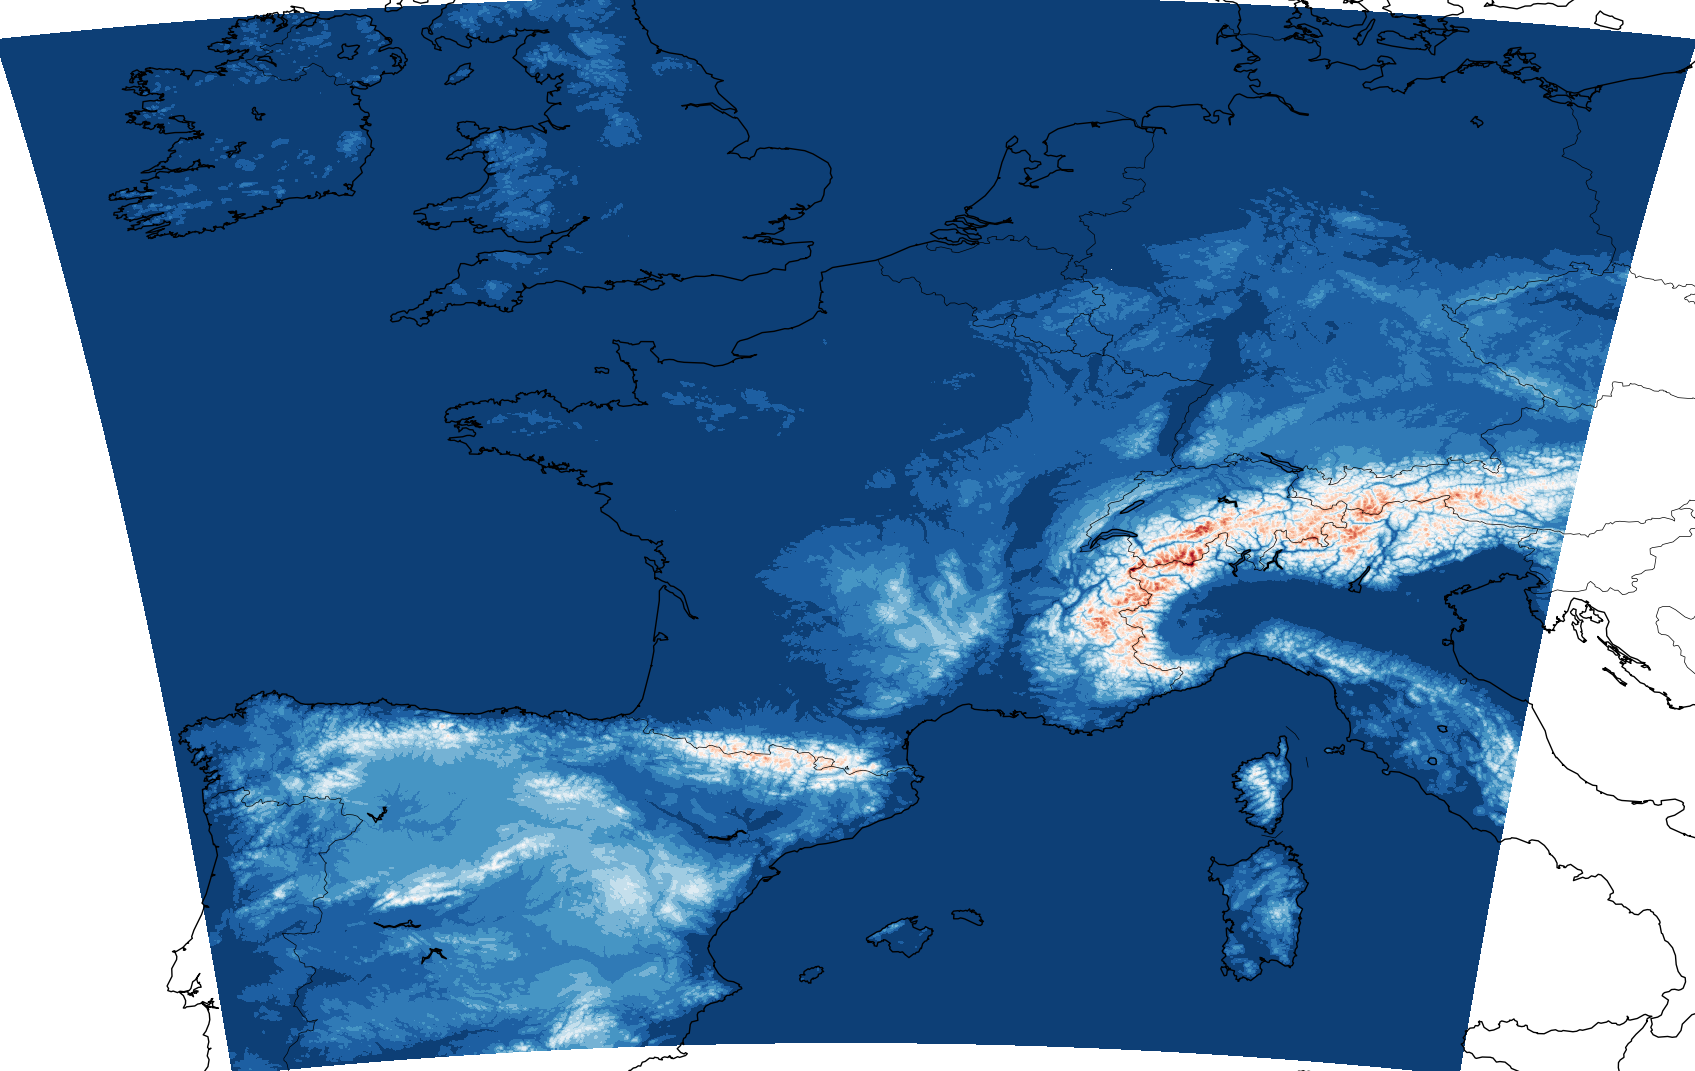
\includegraphics[width=0.5\textwidth]{figures/domaine_calcul_AROME.png}
\end{center}

\hfill\break
\captionof{figure}{\small Cartographie du champ de calcul du modèle numérique AROME.}

\subsubsection{Filtrage des séries
temporelles}\label{filtrage-des-suxe9ries-temporelles}

En chaque point géographique on calcule la part de données manquantes
dans la série temporelle pour chaque saison (ou mois) et année. On
élimine les années dont cette part dépasse le seuil fixé de 10\%. On
déduit le nombre d'années valides restantes. On ne garde que les points
géographiques qui possèdent au moins le nombre minimal d'années exigé
(50 ans pour la période 1959-2022 et 25 ans pour la période 1990-2022).
Les analyses suivantes ne portent plus que sur ce sous‑ensemble de
stations et d'années.

\subsection{Définition des saisons}\label{duxe9finition-des-saisons}

Les saisons sont définies par \textbf{SON} pour septembre (\textbf{SEP})
octobre (\textbf{OCT}) novembre (\textbf{NOV}), \textbf{DJF} pour
décembre (\textbf{DEC}) janvier (\textbf{JAN}) février (\textbf{FEV}),
\textbf{MAM} pour mars (\textbf{MAR}) avril (\textbf{AVR}) mai
(\textbf{MAI}), et \textbf{JJA} pour juin (\textbf{JUI}) juillet
(\textbf{JUILL}) août (\textbf{AOU}). L'année hydrologique
(\textbf{HYDRO}) est définie comme la période allant du 1er septembre de
l'année N au 31 août de l'année N+1.

\subsection{Calcul des indicateurs
descriptifs}\label{calcul-des-indicateurs-descriptifs}

À partir des données obtenues de Météo-France et d'AROME, le nombre de
jour de pluie (seuil fixé à 1 mm/j), le cumul et les maxima de
précipitations journalières et horaires ont été calculées pour chaque
point de grille AROME ou station, année et mois/saison sur les période
1959-2022 et 1990-2022.

\subsection{Vers une généralisation par modélisation
statistique}\label{vers-une-guxe9nuxe9ralisation-par-moduxe9lisation-statistique}

Les statistiques descriptives ne permettent pas d'extrapoler, quantifier
l'incertitude et la significativité et de relier proprement les
tendances observées aux mécanismes physiques. On ne peut donc pas
transformer des constats descriptifs en résultats exploitables et
comparables. Pour répondre à ces questions, nous mobilisons la théorie
des valeurs extrêmes et en particulier le théorème de
Fisher--Tippett--Gnedenko \citep{coles2001introduction}. Les maxima, une
fois normalisés, convergent vers une GEV. C'est l'analogue, pour les
maxima, du théorème central limite pour les sommes. Ce théorème stipule
que, si \((M_n)\) désigne la suite des maxima normalisés d'échantillons
indépendants et identiquement distribués, alors sous des conditions
générales, la loi limite de \(M_n\) appartient à la famille généralisée
des valeurs extrêmes (Generalized Extreme Value, GEV). La GEV unifie
trois familles classiques : Gumbel (\(\xi \to 0\)), Fréchet
(\(\xi > 0\)) et Weibull (\(\xi < 0\)). La \emph{bonne} famille étant
déterminée automatiquement par l'estimation de \(\xi\) qui contrôle la
lourdeur de la queue. Nous ajustons des lois GEV aux maxima, d'abord
dans un cadre stationnaire pour valider le bon comportement du modèle,
puis dans un cadre non‑stationnaire où les paramètres de la GEV
dépendent du temps. Cette étape nous permet de comparer de manière
cohérente les niveaux de retour entre observations et AROME, d'estimer
leurs tendances et de relier ces tendances aux mécanismes physiques.

\subsubsection{Définitions}\label{duxe9finitions}

Si on note \(x\) une réalisation de la variable aléatoire \(X\),
représentant le maximum annuel de précipitations en un point spatial
donné, alors la loi GEV est une loi de probabilité continue paramétrée
par le triplet \(\theta = (\mu, \sigma, \xi)\) --- respectivement la
position, l'échelle (strictement positive) et la forme dont la fonction
de répartition cumulative est :

\[
F(x;\mu ,\sigma ,\xi) = \exp\left\{-\left[1 + \xi\frac{x - \mu}{\sigma}\right]^{-1/\xi}\right\}, \quad 1 + \xi\frac{x - \mu}{\sigma} > 0
\]

\subsubsection{Covariable temporelle}\label{covariable-temporelle}

On dispose d'une série temporelle de \(n\) maxima annuels de
précipitations pour un point géographique. On suppose ces maxima
indépendants. Ces observations sont notées \(\{x_1, x_2, \dots, x_n\}\)
où chaque \(x_i\) est un maximum annuel de précipitations observé à
l'année \(t_i\) et qui suit une loi GEV dont les paramètres dépendent,
analytiquement, de l'année \(i\). On transforme l'année \(t_i\) en une
covariable normalisée notée \(\tilde{t}_i\). Cette transformation est
simplement réalisée pour des raisons numériques mais elle ne change rien
au résultat théorique. On crée également une covariable temporelle avec
point de rupture noté \(t_+\) tel que :

\[
\tilde{t}_i = \frac{t_i - t_{\min}}{t_{\max} - t_{\min}} \quad \text{avec} \quad \begin{cases}
t_{min} = \min_i t_i \\
t_{max} = \max_i t_i
\end{cases} \quad \text{et} \quad
\tilde{t}_{i}^\ast =
\begin{cases}
0 & \text{si } t_i < t_+ \\
\displaystyle \frac{t_i - t_+}{t_{\max} - t_+} & \text{si } t_i \ge t_+
\end{cases}
\]

Ce codage permet d'appliquer une pente temporelle seulement après la
date de rupture, avec une covariable encore normalisée sur \([0,1]\)
dans la portion post-rupture.

\subsubsection{Modèles utilisés}\label{moduxe8les-utilisuxe9s}

\begin{tcolorbox}[enhanced jigsaw, toprule=.15mm, left=2mm, rightrule=.15mm, leftrule=.75mm, breakable, opacityback=0, colback=white, arc=.35mm, bottomrule=.15mm, colframe=quarto-callout-color-frame]

Soit la covariable
\(t \in \mathbb{N} \mid t_{\min} \leq t \leq t_{\max}\). Le modèle
stationnaire est défini par \(M_0(\theta_0)\) et
\(\theta_0 = (\mu_0, \sigma_0, \xi_0)\) avec \(\mu(t) = \mu_0\) ;
\(\sigma(t) = \sigma_0\) ; \(\xi(t) = \xi_0\). Les modèles non
stationnaires sont définis par :

\[
\begin{array}{c@{\qquad}c@{\qquad}c}
% -------- Colonne 1 --------
\begin{array}{c}
\begin{aligned}
M_1(\theta_1)\\[-0.2ex]
\theta_1 = (\mu_0, \mu_1, \sigma_0, \xi_0)
\end{aligned}\\[0.4ex]
\begin{cases}
\mu(t) = \mu_0 + \mu_1\, t \\
\sigma(t) = \sigma_0 \\
\xi(t) = \xi_0
\end{cases}
\end{array}
&
% -------- Colonne 2 --------
\begin{array}{c}
\begin{aligned}
M_2(\theta_2)\\[-0.2ex]
\theta_2 = (\mu_0, \sigma_0, \sigma_1, \xi_0)
\end{aligned}\\[0.4ex]
\begin{cases}
\mu(t) = \mu_0 \\
\sigma(t) = \sigma_0 + \sigma_1\, t \\
\xi(t) = \xi_0
\end{cases}
\end{array}
&
% -------- Colonne 3 --------
\begin{array}{c}
\begin{aligned}
M_3(\theta_3)\\[-0.2ex]
\theta_3 = (\mu_0, \mu_1, \sigma_0, \sigma_1, \xi_0)
\end{aligned}\\[0.4ex]
\begin{cases}
\mu(t) = \mu_0 + \mu_1\, t \\
\sigma(t) = \sigma_0 + \sigma_1\, t \\
\xi(t) = \xi_0
\end{cases}
\end{array}
\end{array}
\]

\end{tcolorbox}

Lorsqu'un point de rupture noté \(t_+\) est introduit, on note :

\[
t^\ast = t \cdot \mathbb{1}_{t > t_+} \quad \text{avec} \quad t_+ \in \mathbb{N}
\]

Les modèles \(M_1\), \(M_2\) et \(M_3\) deviennent respectivements
\(M_1^\ast\), \(M_2^\ast\) et \(M_3^\ast\). Sur cette même notation
\(\theta_i\) devient \(\theta^\ast_i\) avec \(i \in \{1, 2, 3\}\). Dans
cette étude, on réalise les modélisations stationnaire et
non-stationnaires avec pour covariable l'année et un effet temporel sur
\(\mu\) ou \(\sigma\) ou \(\mu\) et \(\sigma\). \(\xi\) est choisi comme
constant. Sur la base bibliographique, on choisi \(t_+ = 1985\). Cette
année de rupture est motivée par plusieurs considérations : 1) des
études précédentes ont montré que les tendances statistiquement
significatives des extrêmes de précipitations quotidiennes dans le sud
de la France commencent dans les années 1980 \citep{Blanchet2018} ; 2)
c'est en ce point que la log-vraisemblance est maximisée
\citep{Blanchet2018}. En utilisant une année de rupture, nous sommes en
mesure de minimiser les potentiels biais découlant des différentes
longueurs d'observations tout en pouvant prendre en compte les données
supplémentaires antérieures à 1985 pour rendre les estimations plus
robustes.

\subsubsection{Niveau de retour}\label{niveau-de-retour}

Le niveau de retour (ou quantile d'ordre \(1 - \tfrac{1}{T}\)) dans une
loi GEV (Figure 3) correspond à une valeur seuil \(z_T\) que l'on
dépasse, en moyenne, une fois tous les \(T\) ans. Soit
\(X \sim \mathrm{GEV}(\mu, \sigma, \xi)\), alors en notant \(F^{-1}\) la
fonction quantile de la GEV, on obtient :

\begin{tcolorbox}[enhanced jigsaw, toprule=.15mm, left=2mm, rightrule=.15mm, leftrule=.75mm, breakable, opacityback=0, colback=white, arc=.35mm, bottomrule=.15mm, colframe=quarto-callout-color-frame]

\[
\mathbb{P}(X > z_T) = \frac{1}{T}, \quad \text{soit} \quad z_T = F^{-1}\left(1 - \frac{1}{T} \right) = 
\begin{cases}
\mu + \frac{\sigma}{\xi} \left[ \left( -\log\left(1 - \frac{1}{T}\right) \right)^{-\xi} - 1 \right] & \text{si } \xi \ne 0 \\
\mu - \sigma \log \left( -\log\left(1 - \frac{1}{T} \right) \right) & \text{si } \xi = 0 \quad \text{(Gumbel)}
\end{cases}
\]

\end{tcolorbox}

\citet{berghald2024caracterisation} montre l'influence des paramètres de
la GEV sur la densité de probabilité et sur la relation entre période et
niveau de retour (Figure 3).

\hfill\break

\begin{center}
  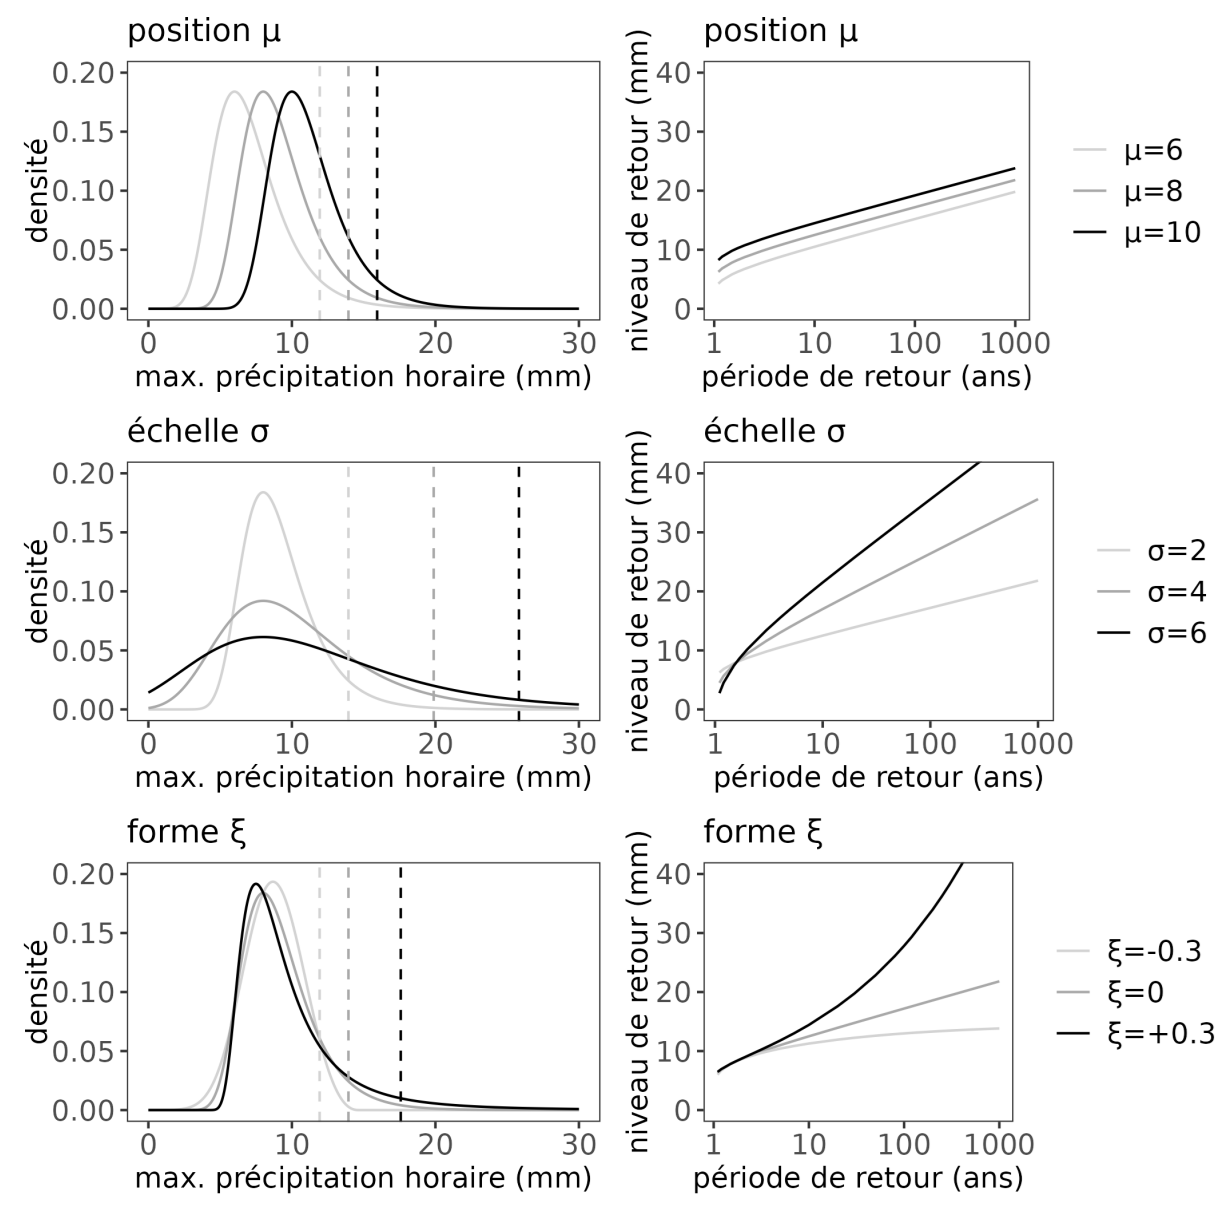
\includegraphics[width=0.6\textwidth]{figures/fig_gev.png}
\end{center}

\captionof{figure}{\small Influence des paramètres de la GEV sur la densité de probabilité (à gauche) et sur la relation entre période et niveau de retour (à droite) : position $\mu$ (en haut), échelle $\sigma$ (centre) et forme $\xi$ (en bas). Les lignes pointillées montrent le niveau de retour de 20\,ans pour les différents cas \cite{berghald2024caracterisation}.}

\subsubsection{Vraisemblance et maximum de
vraisemblance}\label{vraisemblance-et-maximum-de-vraisemblance}

Soit la fonction de vraisemblance
\({\displaystyle {\mathcal {L}}(\theta ;x)} : {\displaystyle \theta \mapsto f(x;\theta )}\).
La log-vraisemblance \(\ell(\theta) = \log \mathcal{L}(\theta)\) s'écrit
après développement (Annexes 1-1) :

\begin{tcolorbox}[enhanced jigsaw, toprule=.15mm, left=2mm, rightrule=.15mm, leftrule=.75mm, breakable, opacityback=0, colback=white, arc=.35mm, bottomrule=.15mm, colframe=quarto-callout-color-frame]

\[
\ell(\theta)=
-\sum_{i=1}^n\Bigl[
\log\sigma
+\Bigl(1+\tfrac1{\xi}\Bigr)\log y_i
+y_i^{-\frac{1}{\xi}}
\Bigr]
\quad \text{avec} \quad  y_i(\theta)=1+\xi\;\frac{x_i-\mu}{\sigma}
\tag{1}
\]

\end{tcolorbox}

On obtient alors :

\[
\scalebox{0.7}{
\(
\begin{aligned}
\ell_{M_0}(\mu_0, \sigma_0, \xi_0) &=
-\sum_{i=1}^n \left[
\log \sigma_0 +
\left(1 + \frac{1}{\xi_0} \right) \log \left(1 + \xi_0 \frac{x_i - \mu_0}{\sigma_0} \right) +
\left(1 + \xi_0 \frac{x_i - \mu_0}{\sigma_0} \right)^{-1/\xi_0}
\right]\\ 
\ell_{M_1}(\mu_0, \mu_1, \sigma_0, \xi_0) &=
-\sum_{i=1}^n \left[
\log \sigma_0 +
\left(1 + \frac{1}{\xi_0} \right) \log \left(1 + \xi_0 \frac{x_i - (\mu_0 + \mu_1 \cdot \tilde{t}_i)}{\sigma_0} \right) +
\left(1 + \xi_0 \frac{x_i - (\mu_0 + \mu_1 \cdot \tilde{t}_i)}{\sigma_0} \right)^{-1/\xi_0}
\right]\\ 
\ell_{M_2}(\mu_0, \sigma_0, \sigma_1, \xi_0) &=
-\sum_{i=1}^n \left[
\log (\sigma_0 + \sigma_1 \tilde{t}_i) +
\left(1 + \frac{1}{\xi_0} \right) \log \left(1 + \xi_0 \frac{x_i - \mu_0}{\sigma_0 + \sigma_1 \tilde{t}_i} \right) +
\left(1 + \xi_0 \frac{x_i - \mu_0}{\sigma_0 + \sigma_1 \tilde{t}_i} \right)^{-1/\xi_0}
\right]\\ 
\ell_{M_3}(\mu_0, \mu_1, \sigma_0, \sigma_1, \xi_0) &=
-\sum_{i=1}^n \left[
\log (\sigma_0 + \sigma_1 \tilde{t}_i) +
\left(1 + \frac{1}{\xi_0} \right) \log \left(1 + \xi_0 \frac{x_i - (\mu_0 + \mu_1 \tilde{t}_i)}{\sigma_0 + \sigma_1 \tilde{t}_i} \right) +
\left(1 + \xi_0 \frac{x_i - (\mu_0 + \mu_1 \tilde{t}_i)}{\sigma_0 + \sigma_1 \tilde{t}_i} \right)^{-1/\xi_0}
\right]
\end{aligned}
\tag{1'}
\)
}
\]

Les vraisemblances de \(M_1^*, M_2^*, M_3^*\) sont obtenues en
remplaçant \(\tilde{t}_i\) par \(\tilde{t}_i^\ast\) dans les expressions
ci-dessus.

En pratique, les paramètres \((\mu, \sigma, \xi)\) sont inconnus et
estimés à partir des données par un estimateur
\(\hat{\theta} = (\hat{\mu}, \hat{\sigma}, \hat{\xi})\) obtenu par
maximum de vraisemblance (MLE) via une optimisation numérique tel que
\(\hat{\theta} = \arg\max_{\theta} \, \ell(\theta)\). Il n'existe pas de
formule explicite des paramètres, ceux-ci étant déterminés numériquement
en maximisant la vraisemblance.

L'estimateur du niveau de retour \(\hat{z}_T\) s'écrit alors
\(\hat{z}_{T}\;=\;F^{-1}_{\hat{\theta}}\!\left(1-\frac{1}{T}\right)\).
Le MLE classique donne un point estimé, mais pas d'intervalle. On
souhaite aussi connaître l'incertitude autour de l'estimation de
\(\hat{z}_T\). Pour cela, on utilise la vraisemblance profilée.

\subsubsection{Vraisemblance profilée et intervalle de confiance d'un
niveau de
retour}\label{vraisemblance-profiluxe9e-et-intervalle-de-confiance-dun-niveau-de-retour}

\(z_T\) peut se réecrire sous la forme
\(\mu = z_T - \dfrac{\sigma}{\xi} \left[ \left( -\log\left(1 - \frac{1}{T} \right) \right)^{-\xi} - 1 \right]\).
La combinaison des paramètres temporels de la loi GEV conduit à une
expression linéaire en \(t\) :

\[
z_T(t) = z_{T,0} + z_{T,1} \cdot t
\]

En développant les paramètres soumis à un effet temporel et on
regroupant terme à terme on peut montrer que (Annexes 1-2) :

\[
\mu_1(z_{T,1}) = z_{T,1} -\dfrac{\hat{\sigma_1}}{\hat{\xi}_0}\Bigl(\bigl[-\log(1-\tfrac1T)\bigr]^{-\hat{\xi}_0}-1\Bigr) \quad \text{et} \quad
\sigma_1(z_{T,1}) = \dfrac{\hat{\xi}_0\,\bigl(z_{T,1}-\hat{\mu_1}\bigr)}{\bigl[-\log\!\bigl(1-\tfrac1T\bigr)\bigr]^{-\hat{\xi}_0}-1}
\]

On cherche l'intervalle de confiance sur \(z_{T,1}\) donc pour chaque
valeur candidate \(z_{T,1}\) dans une grille (autour de l'estimateur
\(\hat{z}_{T,1}\)), on maximise les log-vraisemblances (1') qui
deviennent des log-vraisemblances profilées \(\ell^{\,p}\) :

\[
\scalebox{0.7}{
\(
\begin{aligned}
\underset{\hat{\sigma}_1 = 0}{\ell_{M_1}^{\,p}(z_{T,1} \ ; \hat{\mu}_0, \hat{\sigma}_0, \hat{\xi}_0)} &= 
-\sum_{i=1}^n \left[
\log \hat{\sigma}_0 +
\left(1 + \frac{1}{\hat{\xi}_0} \right) \log \left(1 + \hat{\xi}_0 \frac{x_i - (\hat{\mu}_0 + \mu_1(z_{T,1}) \cdot \tilde{t}_i)}{\hat{\sigma}_0} \right) +
\left(1 + \hat{\xi}_0 \frac{x_i - (\hat{\mu}_0 + \mu_1(z_{T,1}) \cdot \tilde{t}_i)}{\hat{\sigma}_0} \right)^{-1/\hat{\xi}_0}
\right]\\
\underset{\hat{\mu}_1 = 0}{\ell_{M_2}^{\,p}(z_{T,1} \ ; \hat{\mu}_0, \hat{\sigma}_0, \hat{\xi}_0)} &= 
-\sum_{i=1}^n \left[
\log (\hat{\sigma}_0 + \sigma_1(z_{T,1}) \cdot \tilde{t}_i) +
\left(1 + \frac{1}{\hat{\xi}_0} \right) \log \left(1 + \hat{\xi}_0 \frac{x_i - \hat{\mu}_0}{\hat{\sigma}_0 + \sigma_1(z_{T,1}) \cdot \tilde{t}_i} \right) +
\left(1 + \hat{\xi}_0 \frac{x_i - \hat{\mu}_0}{\hat{\sigma}_0 + \sigma_1(z_{T,1}) \cdot \tilde{t}_i} \right)^{-1/\hat{\xi}_0}
\right]\\
\ell_{M_3}^{\,p}(z_{T,1} \ ; \hat{\mu}_0, \hat{\sigma}_0, \hat{\sigma}_1, \hat{\xi}_0) &= 
-\sum_{i=1}^n \left[
\log (\hat{\sigma}_0 + \hat{\sigma}_1 \tilde{t}_i) +
\left(1 + \frac{1}{\hat{\xi}_0} \right) \log \left(1 + \hat{\xi}_0 \frac{x_i - (\hat{\mu}_0 + \mu_1(z_{T,1}) \tilde{t}_i)}{\hat{\sigma}_0 + \hat{\sigma}_1 \tilde{t}_i} \right) +
\left(1 + \hat{\xi}_0 \frac{x_i - (\hat{\mu}_0 + \mu_1(z_{T,1}) \tilde{t}_i)}{\hat{\sigma}_0 + \hat{\sigma}_1 \tilde{t}_i} \right)^{-1/\hat{\xi}_0}
\right]\\
\end{aligned}
\tag{2}
\)
}
\]

On cherche donc :

\[
\hat{z}_{T,1} = \underset{z_{T,1}}{\arg\max} \; \ell_{M_\bullet}^{\,p}(z_{T,1} \ ; \hat{\theta}_{\bullet}) \quad \text{avec} \quad
\hat{\theta}_{\bullet} = \begin{cases}
\hat{\theta}_{1}^{\,p} = (\hat{\mu_0}, \hat{\sigma_0}, \hat{\xi_0}) & \text{pour } M_1 \\
\hat{\theta}_2^{\,p} = (\hat{\mu_0}, \hat{\sigma_0}, \hat{\xi_0}) & \text{pour } M_2 \\
\hat{\theta}_3^{\,p} = (\hat{\mu_0}, \hat{\sigma_0}, \hat{\sigma_1}, \hat{\xi_0}) & \text{pour } M_3 \\
\end{cases}
\]

On trace ainsi pour chaque modèle \(M_\bullet\) la fonction
\({\displaystyle \mathcal{L}_{M_\bullet} : z_{T,1} {\mapsto} \ell_{M_\bullet}^{\,p}(z_{T,1} \ ; \hat{\theta}_{\bullet})}\)

L'intervalle de confiance de \(\hat{z}_{T,1}\) pour un modèle
\(M_\bullet\) au seuil \((1 - \alpha)\) basé sur le profil de
vraisemblance est donné par :

\[
\operatorname{IC}_{M_\bullet}^{(1-\alpha)}\!\bigl(\hat{z}_{T,1}\bigr)
   = \Bigl\{\, z_{T,1}\;:\;
        2\bigl[\ell_{M_\bullet}^{\,p}(\hat{z}_{T,1} \ ; \hat{\theta}_{\bullet})-\ell_{M_\bullet}^{\,p}(z_{T,1} \ ; \hat{\theta}_{\bullet})\bigr]
        \le \chi^{2}_{1,\,1-\alpha} \Bigr\}
\]

où \(\chi^2_{1,1-\alpha}\) est le quantile d'ordre \(1 - \alpha\) d'une
loi du \(\chi^2\) à un degré de liberté. On fixe ici \(\alpha=0{,}10\).
Lorsque l'intervalle de confiance ne contient pas 0 alors
\(\hat{z}_{T,1}\) est significatif.

\subsection{Choix du meilleur modèle}\label{choix-du-meilleur-moduxe8le}

\subsubsection{Test du rapport de vraisemblance
(LRT)}\label{test-du-rapport-de-vraisemblance-lrt}

En tout point géographique on dispose de
\(M_0, M_1, M_2, M_3, M_1^\ast, M_2^\ast \text{ et } M_3^\ast\). Notons
\(k_j\) le nombre de paramètres du modèle \(M_j\). On souhaite tester,
pour chaque modèle non stationnaire \(j \neq 0\), l'hypothèse nulle
\(H_0\) : \(M_j\) ne~fait~pas~mieux~que \(M_0\) (stationnarité). Pour
chaque modèle non stationnaire \(j\neq 0\) et chaque point \(i\) en
notant \(p_{ij}\) la \(p\)-valeur\,:

\[
\Lambda_{ij}=2\bigl(\ell_{ij}-\ell_{i0}\bigr) \overset{H_0}{\sim}\chi^{2}_{\;k_j-k_0} \quad \text{avec} \quad p_{ij}= \mathbb{P}(\chi^{2}_{k_j-k_0}\ge \Lambda_{ij}\bigr)
\]

\subsubsection{Règle hiérarchique de
sélection}\label{ruxe8gle-hiuxe9rarchique-de-suxe9lection}

Soit \(\alpha=0{,}10\) le seuil d'intérêt. Si un des deux modèles
\(M_3\) ou \(M_3^\ast\) vérifie \(p_{ij}\le\alpha\), on retient
\(j=\arg\min_{j\in\{3,3^\ast\}} p_{ij}\). Sinon, on compare l'ensemble
des six modèles non stationnaires et l'on sélectionne
\(j=\arg\min_{j\in\{1,1^\ast,2,2^\ast,3,3^\ast\}} p_{ij}\). Cette double
étape privilégie les formes \emph{simultanément} temporelles sur \(\mu\)
et \(\sigma\) quand elles sont statistiquement justifiées. Cela assure
que la complexité n'est introduite que lorsqu'elle apporte une
information statistiquement crédible tout en livrant, pour chaque poste,
un modèle non stationnaire.

\subsection{Calcul des tendances}\label{calcul-des-tendances}

A partir des niveaux de retour 10 ans (\(T = 10\)) la tendance relative
(en \%) entre 1995 et 2022 est calculée via la formule ci-dessous. Un
exemple graphique est disponible en annexes 2-6.

\begin{tcolorbox}[enhanced jigsaw, toprule=.15mm, left=2mm, rightrule=.15mm, leftrule=.75mm, breakable, opacityback=0, colback=white, arc=.35mm, bottomrule=.15mm, colframe=quarto-callout-color-frame]

\[
\text{Tendance} = \frac{z_T^{2022} - z_T^{1995}}{z_T^{1995}} \cdot {100}
\]

\end{tcolorbox}

\subsection{Concordance}\label{concordance}

On évalue l'accord entre les statistiques descriptives et les tendances
obtenues à partir des simulations du modèle AROME et celles observées
dans la réalité. Pour ce faire, chaque station Météo-France est associée
au point de grille AROME (2,5 km × 2,5 km) correspondant à sa
localisation géographique. Cette correspondance permet de calculer la
corrélation de Pearson (\emph{r}) ainsi que l'erreur moyenne (\emph{ME})
entre les valeurs observées et simulées.

\subsection{Représentation
cartographique}\label{repruxe9sentation-cartographique}

Pour homogénéiser les amplitudes extrêmes entre jeux de données (AROME
et données observées), on applique une saturation de couleur suivant la
période étudiée. Soit une période
\(P \in \{\text{HYDRO}, \text{DJF},\text{MAM},\text{JJA},\text{SON}\}\)
ou
\(P \in \{\text{JAN},\text{FEV},\text{MAR},\text{...},\text{OCT},\text{NOV},\text{DEC}\}\).
Pour chaque statistique (nombre de jour de pluie, cumul, moyenne des
maxima, tendance relative) \(T_j\) avec \(j \in P\), on calcule le
\emph{q}-ième percentile des valeurs absolues :

\[
s_j(P)=\operatorname{Quantile}_{q}\big(|T_j|\big)
\]

Le seuil commun de la période \(P\) est défini par
\(S(P)=\max_j s_j(P)\). On remplace ensuite, pour toute valeur
\(x\in T_j\),
\(x \;\leftarrow\; \operatorname{sign}(x)\,\min\big(|x|,\,S(P)\big)\).

On fixe \(q\) de la manière suivante :

\begin{itemize}
\tightlist
\item
  Pour le nombre de jour de pluie : \(q = 99,9\) pour l'échelle
  journalière 1959-2022, 1990-2022 et l'échelle horaire 1990-2022.
\item
  Le cumul et la moyenne des maxima de précipitations : \(q = 99,0\)
  pour l'échelle journalière 1959-2022, 1990-2022 et l'échelle horaire
  1990-2022.
\item
  La tendance relative : \(q = 99,0\) pour l'échelle journalière
  1959-2022 et 1990-2022 et \(q = 90,0\) pour l'échelle horaire
  1990-2022.
\end{itemize}

Les courbes de niveaux 400 et 800m sont représentées en trait fin.

\section{Résultats}\label{ruxe9sultats}

Nous commençons par évaluer, point de grille par point de grille, la
capacité d'AROME à reproduire le régime de précipitations observé par
les stations Météo‑France. Cette première étape stationnaire sert
d'évaluation de qualité avant d'étudier les tendances des niveaux de
retour.

\subsection{Évaluation de la climatologie des précipitations simulées
par
AROME}\label{uxe9valuation-de-la-climatologie-des-pruxe9cipitations-simuluxe9es-par-arome}

Afin d'apprécier la capacité d'AROME à restituer la climatologie des
précipitations, différents indicateurs sont confrontées aux observations
de stations pour une saison donnée : 1) le nombre de jours de pluie
(seuil\,≥\,1\,mm/j) ; 2) le cumul des précipitations ; et 3) la moyenne
des maxima des précipitations.

\subsubsection{Distribution spatiale}\label{distribution-spatiale}

La distribution spatiale des indicateurs d'AROME au regard des
observations permet de : 1) valider et diagnostiquer le modèle en
localisant les biais et vérifier la structure spatiale (gradients et
effets orographiques) ; et 2) comprendre les processus physique
(distinguer les régimes (méditerranéen, alpin, plaine) et voir où AROME
surestime l'orographique ou sous-estime les convectifs intenses).

\paragraph{Nombre de jours de
précipitations}\label{nombre-de-jours-de-pruxe9cipitations}

Sur la période 1959-2022 (Figure 4, colonne de gauche), AROME surestime
légèrement la fréquence annuelle des jours de précipitation : +6.35
jours/an (soit +5.56\%). Des biais locaux marqués subsistent
toutefois\,: plus de +30 jours pour plusieurs stations du Massif central
et des Pyrénées, tandis que des biais négatifs (−10 à −30 jours) se
concentrent dans les Alpes du Nord, le Finistère et l'Alsace. La
corrélation spatiale est élevée (\emph{r =} 0.95), indiquant que le
modèle reproduit correctement les grands gradients régionaux. AROME et
les observations s'accordent pour situer les fréquences maximales sur
les massifs montagneux (Alpes, Pyrénées, Massif central, Vosges, Jura),
avec plus de 140--160 jours/an, et des valeurs également élevées sur le
Grand Ouest atlantique (Bretagne, Normandie, Pays de la Loire\,: 80--120
jours/an). À l'inverse, la façade méditerranéenne et le pourtour
provençal restent les plus secs en fréquence, souvent \textless\,50--70
jours/an.

\setlength{\tabcolsep}{0pt}

\begin{longtable}[]{@{}
  >{\centering\arraybackslash}p{(\linewidth - 6\tabcolsep) * \real{0.2500}}
  >{\centering\arraybackslash}p{(\linewidth - 6\tabcolsep) * \real{0.2500}}
  >{\centering\arraybackslash}p{(\linewidth - 6\tabcolsep) * \real{0.2500}}
  >{\centering\arraybackslash}p{(\linewidth - 6\tabcolsep) * \real{0.2500}}@{}}
\toprule\noalign{}
\begin{minipage}[b]{\linewidth}\centering
\small Nombre de jours par an de précipitations
\end{minipage} & \begin{minipage}[b]{\linewidth}\centering
\small Cumul annuel des précipitations
\end{minipage} & \begin{minipage}[b]{\linewidth}\centering
\small Moyenne des maxima journaliers des précipitations
\end{minipage} & \begin{minipage}[b]{\linewidth}\centering
\small Moyenne des maxima horaires des précipitations
\end{minipage} \\
\midrule\noalign{}
\endhead
\bottomrule\noalign{}
\endlastfoot
\pandocbounded{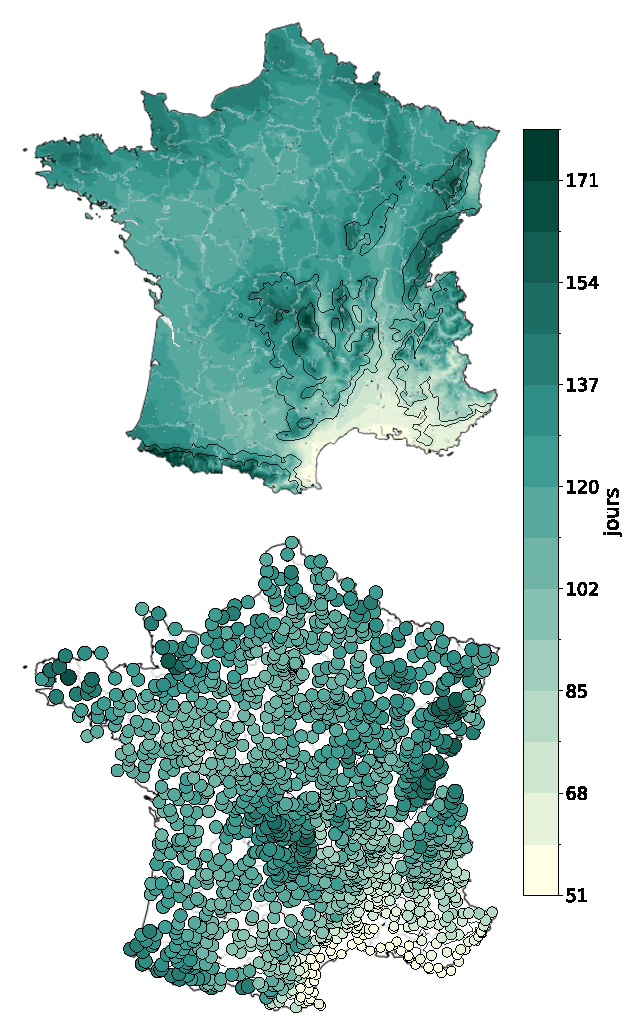
\includegraphics[keepaspectratio]{figures/jour_pluie.pdf}}
&
\pandocbounded{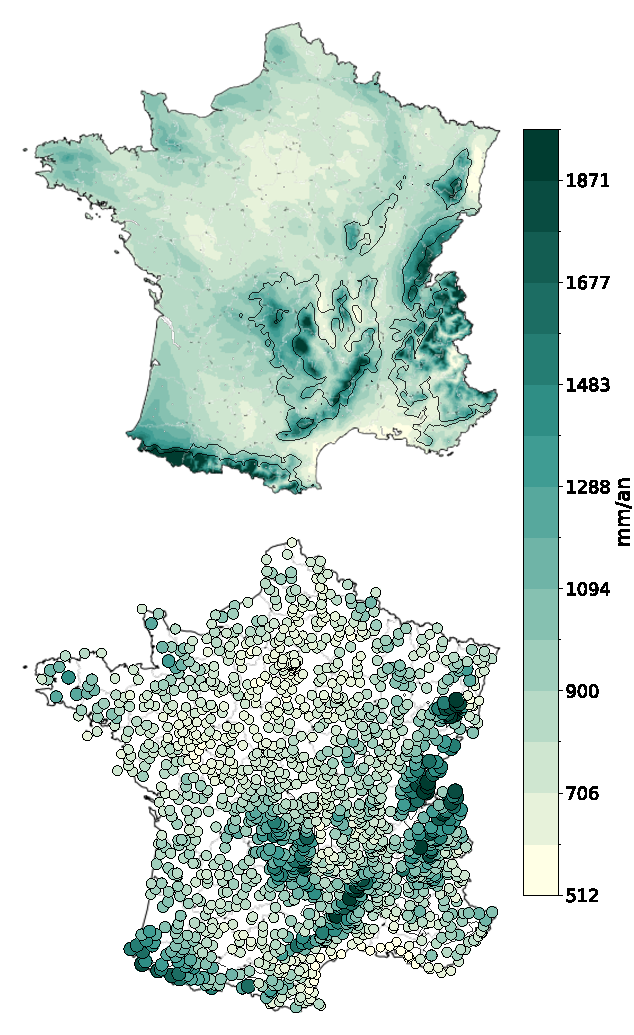
\includegraphics[keepaspectratio]{figures/mean_pluie_jour.pdf}}
&
\pandocbounded{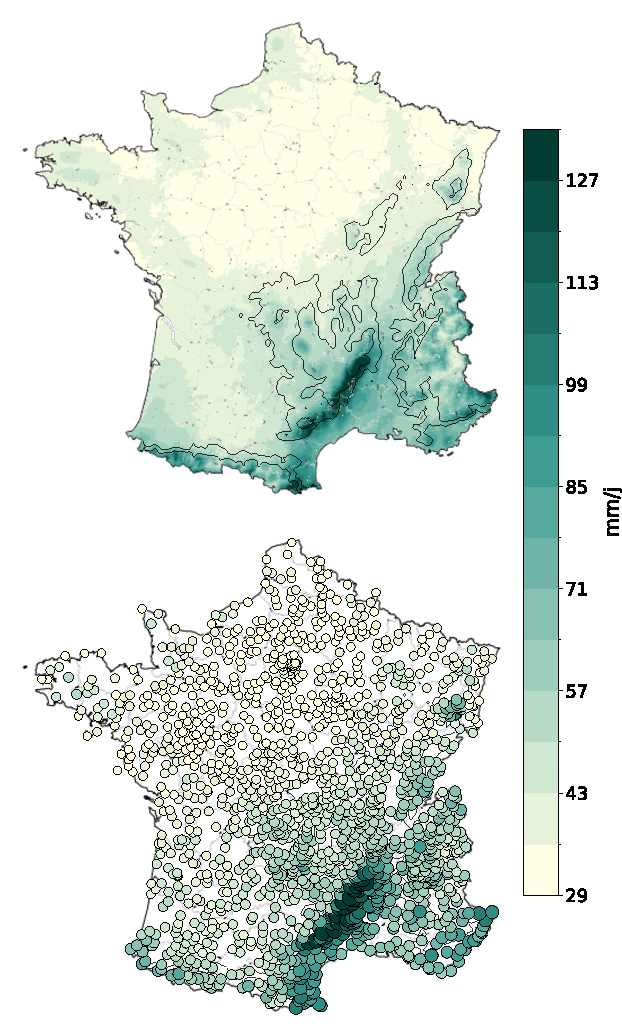
\includegraphics[keepaspectratio]{figures/mean-max_pluie_jour.pdf}}
&
\pandocbounded{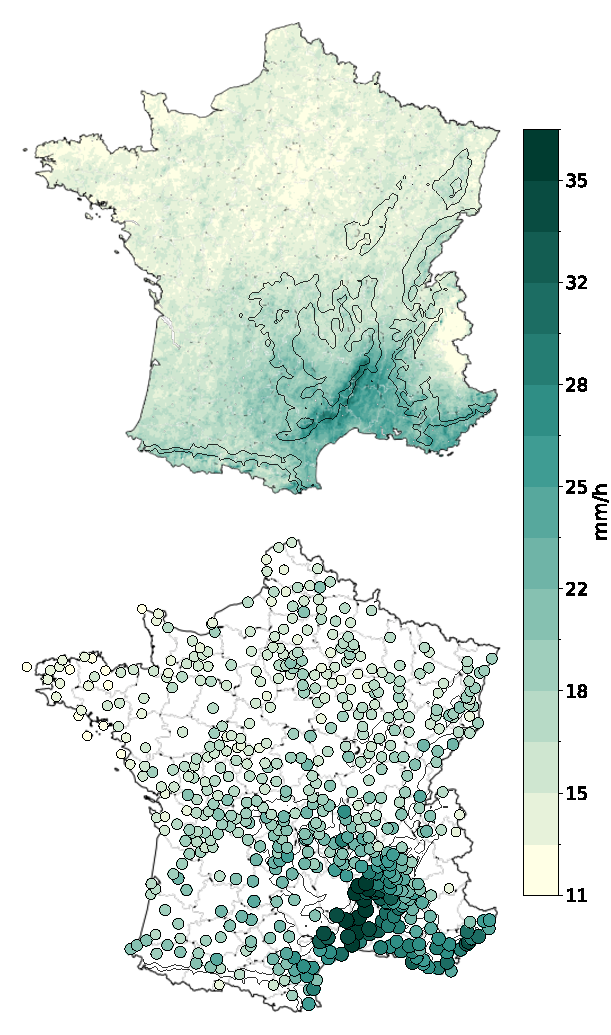
\includegraphics[keepaspectratio]{figures/mean-max_pluie_horaire.pdf}} \\
\small \(r =\) 0.95 (n = 1583) & \small \(r =\) 0.94 (n = 1583) &
\small \(r =\) 0.96 (n = 1583) & \small \(r =\) 0.89 (n = 574) \\
\pandocbounded{\includegraphics[keepaspectratio]{../outputs/maps/stats_numday/quotidien/compare_1/sat_99.9/hydro/obs_rast_diff.pdf}}
&
\pandocbounded{\includegraphics[keepaspectratio]{../outputs/maps/stats_mean/quotidien/compare_1/sat_99.0/hydro/obs_rast_diff.pdf}}
&
\pandocbounded{\includegraphics[keepaspectratio]{../outputs/maps/stats_mean-max/quotidien/compare_5/sat_99.0/hydro/obs_rast_diff.pdf}}
&
\pandocbounded{\includegraphics[keepaspectratio]{../outputs/maps/stats_mean-max/horaire/compare_5/sat_99.0/hydro/obs_rast_diff.pdf}} \\
\small \(ME =\) +6.35 j ~(+5.56\%) & \small \(ME =\) +11.48 mm/an
(+1.23\%) & \small \(ME =\) -1.18 mm/j (-2.35\%) & \small \(ME =\) -3.42
mm/j (-18.65\%) \\
\end{longtable}

\captionof{figure}{\small Climatologie entre le modèle AROME (première ligne), les stations Météo-France (deuxième ligne) avec la corrélation ($r$) et le nombre de stations comparés (n) ainsi que la différence AROME-Station (troisième ligne) avec le biais ($ME$) et l'écart relatif (\%) associé issues de données journalières allant de 1959 à 2022 pour une année hydrologique.}

\paragraph{Cumul annuel des
précipitations}\label{cumul-annuel-des-pruxe9cipitations}

Sur la période 1959-2022 (Figure 4, colonne du centre), AROME estime
correctement le cumul annuel des précipitations : +11.48 mm/an (soit
+1.23\%). Des biais locaux marqués subsistent toutefois\,: plus de +1,0
mm/j pour l'ensemble des stations de la crête pyrénéenne et de la
station de Chamonix, tandis que des biais négatifs (−0,5 à −1,5 mm/j) se
concentrent dans les Alpes du Nord, la côte basque et l'Alsace. La
corrélation spatiale est élevée (\emph{r =} 0.94), indiquant que le
modèle reproduit correctement les grands gradients régionaux. La bordure
atlantique sud‑ouest (Pyrénées, Aquitaine) et les Alpes du Nord
reçoivent les plus forts cumuls (plus de 5\,mm/j). Le Massif central et
les reliefs intérieurs (Vosges, Jura) présentent des cumuls
intermédiaires (2,5-4 mm/j). Le pourtour méditerranéen (Languedoc,
Provence) reste globalement plus sec (\textless{} 1,5 mm/j), malgré des
pluies intenses ponctuelles. Ces résultats sont identiques avec les
données horaires de 1990 à 2022 (Annexe 2-2.3).

\paragraph{Moyenne des maxima des
précipitations}\label{moyenne-des-maxima-des-pruxe9cipitations}

Sur la période 1959-2022 (Figure 4, colonne de droite), AROME
sous-estime légèrement la moyenne des maxima journaliers des
précipitations : -1.18 mm/j (soit -2.35\%). Il subsiste d'importants
biais locaux : déficits de −5 à moins de −20 mm/j sur l'ensemble des
Cévennes et se prolongeant vers l'extrimité Nord des Alpes du Nord, sur
la côté sud-est et la côte basque ; jusqu'à -5 mm/j sur une large partie
du centre de la France et de l'Alsace ; de +5 à +20 mm/j sur la crête
pyrénéennes, les contreforts ouest des Cévennes et les Alpes du Nord. La
corrélation spatiale est élevée (\emph{r =} 0.96), indiquant que le
modèle reproduit correctement les grands gradients régionaux. Les plus
fortes précipitations quotidiennes moyennes se rencontrent dans les
Cévennes et plus généralement sur la face sud-est du Massif central
(environ 100--125\,mm/j). Les reliefs alpins et pyrénéens montrent aussi
des maxima élevés (80--100\,mm/j). La façade atlantique et le bassin
parisien présentent des maxima plus modérés (30--60\,mm/j), tandis que
la Provence et la Côte d'Azur, malgré une fréquence moindre, peuvent
localement connaître de très gros orages (40--80\,mm/j en moyenne).

\hfill\break

Ces premiers résultats, marqués par des biais locaux importants sur les
maxima journaliers, nous conduisent à descendre au pas de temps horaire
(Figure 4). Sur la période 1990-2022, AROME sous-estime fortement la
moyenne des maxima horaires des précipitations : -3.42 mm/h (soit
-18.65\%). Il subsiste d'importants biais : déficits de −5 à moins de
−10 mm/h sur presque l'ensemble de la France mais surtout dans les
Cévennes et la vallée du Rhône. La corrélation spatiale reste élevée
(\emph{r =} 0.89), attestant d'une bonne restitution des grands
gradients déjà observés au pas journalier. Au regard des saisons
(Annexes 2-3.3), le biais s'étend de -0,02 mm/h (DJF) à -3,75 mm/h
(JJA), suggérant une sous‑représentation marquée des extrêmes convectifs
estivaux.

\subsubsection{Corrélation entre le modèle AROME et les stations
Météo-France}\label{corruxe9lation-entre-le-moduxe8le-arome-et-les-stations-muxe9tuxe9o-france}

Quel que soit l'indicateur (Figure 6), le modèle AROME reproduit
fidèlement les observations, avec une corrélation minimale de 0,70.
Indépendamment de l'échelle temporelle retenue\,---\,journalière
(1959‑2022 ou 1990‑2022) ou horaire (1990‑2022)\,---\,et de la saison,
les champs simulés s'accordent très bien avec les données mesurées\,: la
corrélation varie entre 0,92 et 0,98 pour le nombre de jours de pluie et
le cumul des précipitations.

Cette performance se maintient pour la moyenne des maxima journaliers
(périodes 1959‑2022 et 1990‑2022) sur l'année hydrologique, l'automne,
l'hiver et le printemps, mais elle se dégrade en été, avec une
corrélation de 0,85. À l'échelle horaire, la qualité de l'estimation des
maxima se détériore encore\,: la corrélation baisse de 0,4 à 0,8\,point
selon la saison pour l'année hydrologique, l'automne et l'hiver, et
chute à 0,70 au printemps et en été.

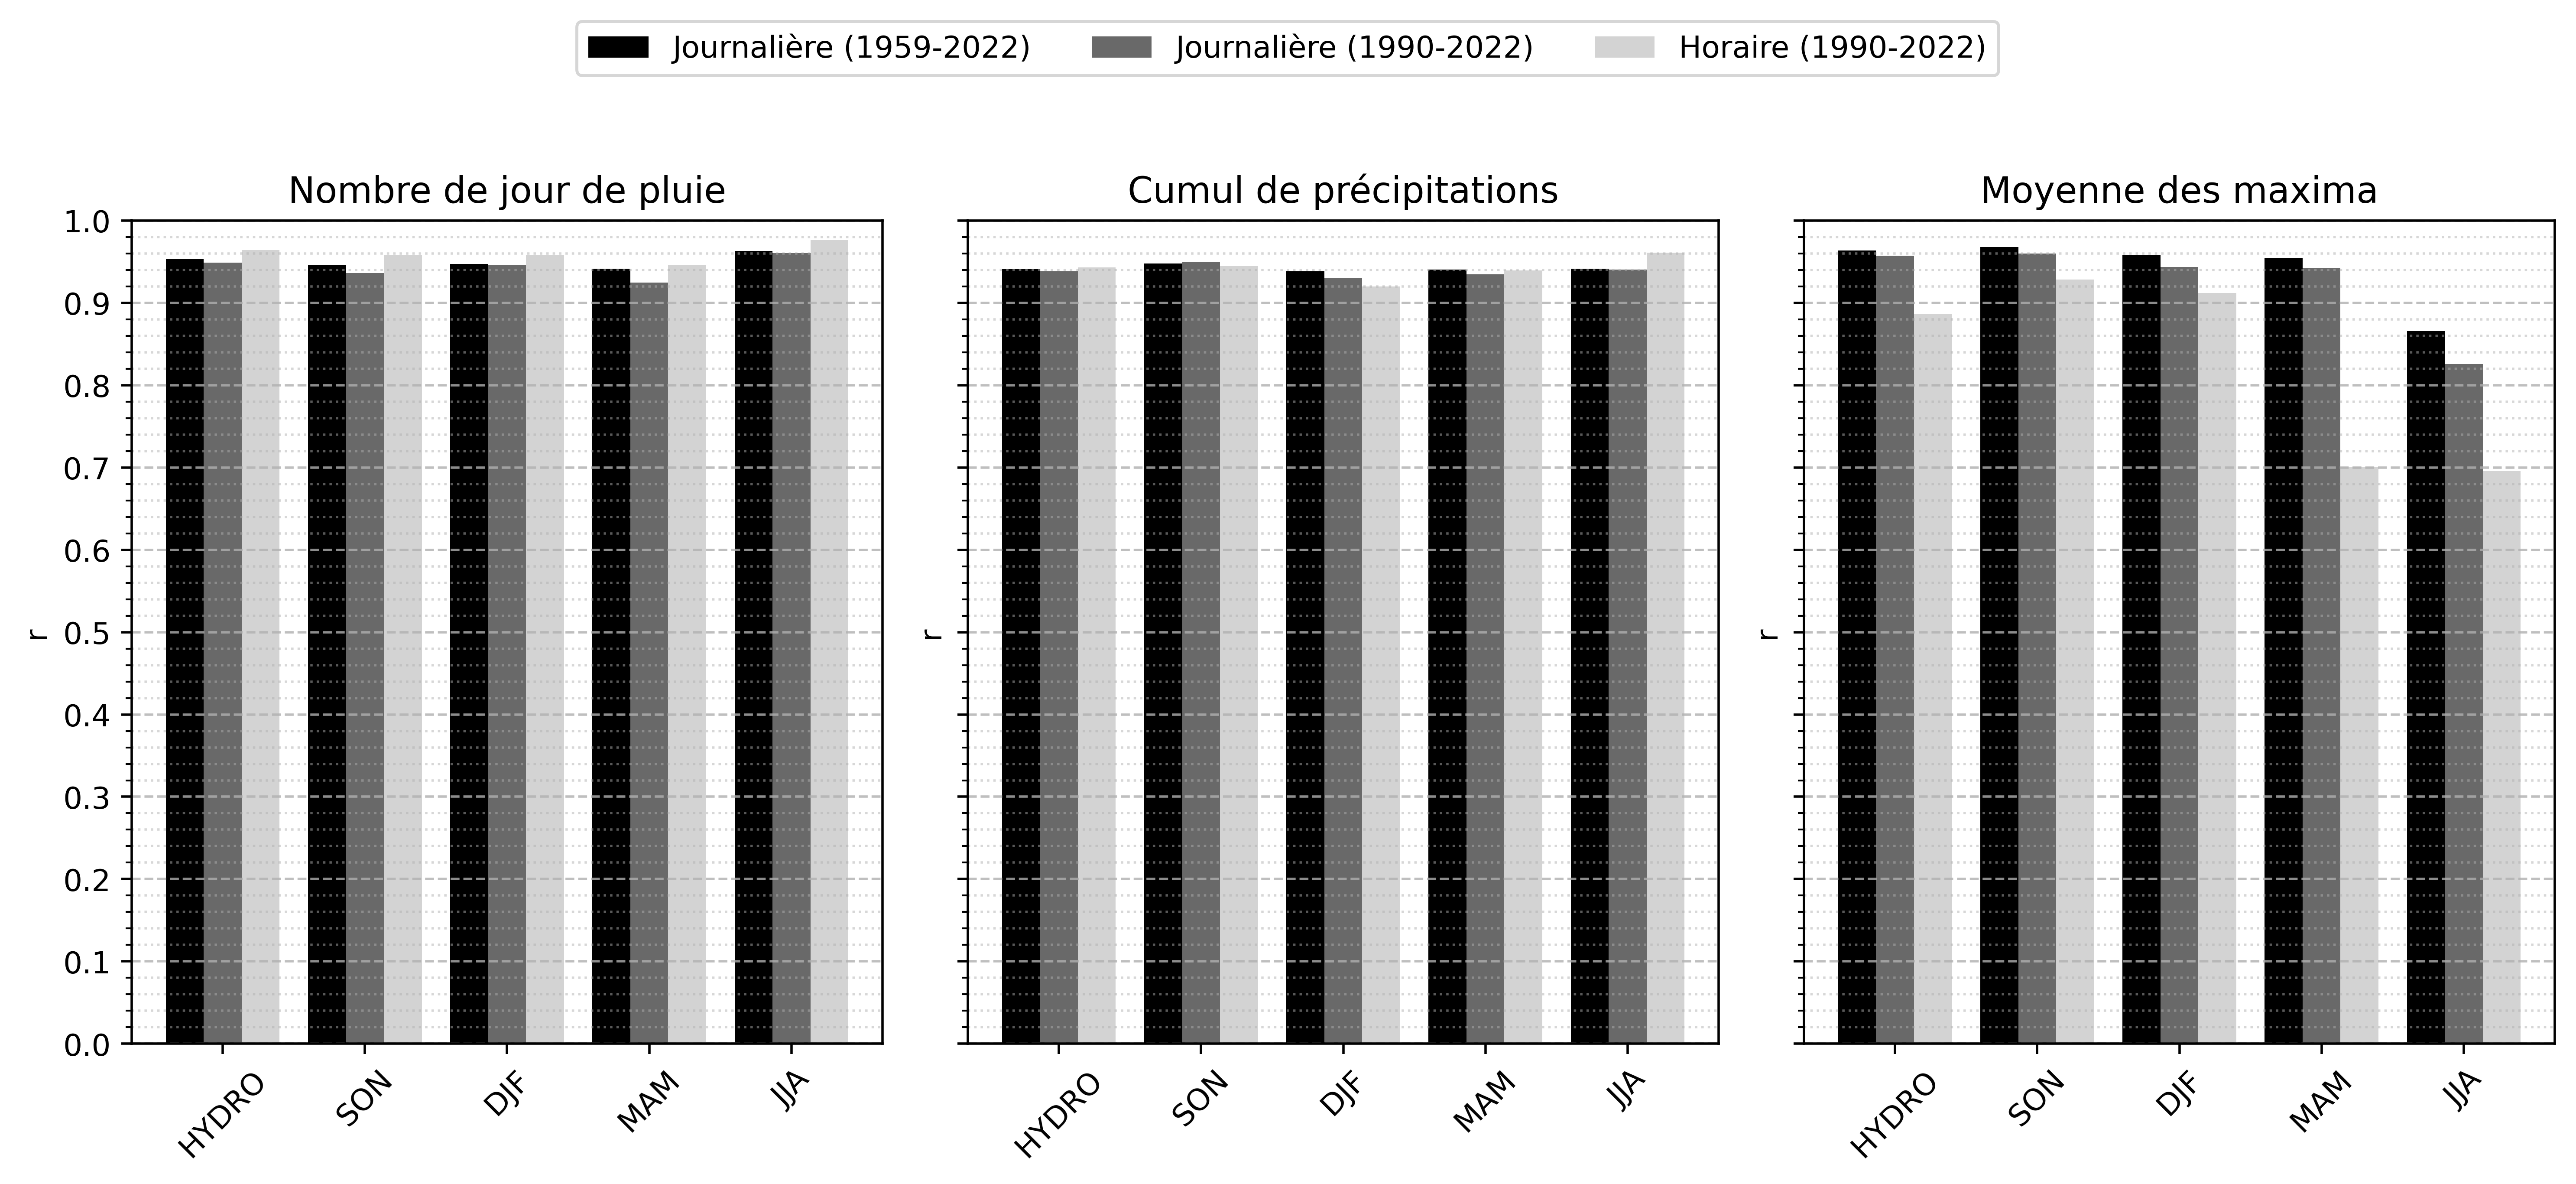
\includegraphics[width=1\linewidth,height=\textheight,keepaspectratio]{figures/histo_numday_mean_mean-max.png}

\captionof{figure}{\small Corrélations des données climatologiques entre le modèle AROME et les stations Météo-France pour chacune des sources de données.}

\begin{tcolorbox}[enhanced jigsaw, toprule=.15mm, left=2mm, rightrule=.15mm, leftrule=.75mm, breakable, opacityback=0, colback=white, arc=.35mm, bottomrule=.15mm, colframe=quarto-callout-color-frame]

AROME sous‑représente les extrêmes convectifs estivaux, surtout à
l'échelle horaire, malgré une structure spatiale bien captée.

\end{tcolorbox}

\subsection{Evaluation des tendances des précipitations
extrêmes}\label{evaluation-des-tendances-des-pruxe9cipitations-extruxeames}

Nous évaluons à présent les tendances des niveaux de retour décennaux
(T\,=\,10\,ans) \emph{significatifs} des précipitations, en visualisant
leur hétérogénéité spatiale et saisonnière et en quantifiant leur
amplitude et leur significativité statistique afin d'identifier les
régions et périodes où l'intensification des extrêmes est la plus
marquée.

\subsubsection{Distribution spatiale}\label{distribution-spatiale-1}

Comme précédemment on commence par analyser la distribution spatiale des
tendances d'AROME au regard des observations.

\paragraph{Données journalières}\label{donnuxe9es-journaliuxe8res}

Nous commençons par vérifier que notre méthodologie restitue bien les
tendances déjà établies à l'échelle journalière sur 1959‑2022 ---
période longue, largement documentée --- de façon à valider les signaux
avant de descendre au pas horaire.

Les tendances relatives de 1995 à 2022 estimées avec AROME sont
spatialement hétérogènes (Annexes\,2‑4.1.1.2, \textbf{HYDRO}). Seul le
Mercantour se distingue par une hausse significative comprise entre +20
et +30\,\%. Les stations montrent par ailleurs un signal positif
généralisé le long de la vallée du Rhône, avec des tendances de +5 à
\textgreater+30\,\%. Hors de ces zones, les tendances sont faibles, de
signe variable et le plus souvent non significatives, ce qui plaide pour
une analyse saisonnière (Figure 7).

\setlength{\tabcolsep}{0pt}

\begin{longtable}[]{@{}
  >{\centering\arraybackslash}p{(\linewidth - 6\tabcolsep) * \real{0.2500}}
  >{\centering\arraybackslash}p{(\linewidth - 6\tabcolsep) * \real{0.2500}}
  >{\centering\arraybackslash}p{(\linewidth - 6\tabcolsep) * \real{0.2500}}
  >{\centering\arraybackslash}p{(\linewidth - 6\tabcolsep) * \real{0.2500}}@{}}
\toprule\noalign{}
\begin{minipage}[b]{\linewidth}\centering
\small SON
\end{minipage} & \begin{minipage}[b]{\linewidth}\centering
\small DJF
\end{minipage} & \begin{minipage}[b]{\linewidth}\centering
\small MAM
\end{minipage} & \begin{minipage}[b]{\linewidth}\centering
\small JJA
\end{minipage} \\
\midrule\noalign{}
\endhead
\bottomrule\noalign{}
\endlastfoot
\pandocbounded{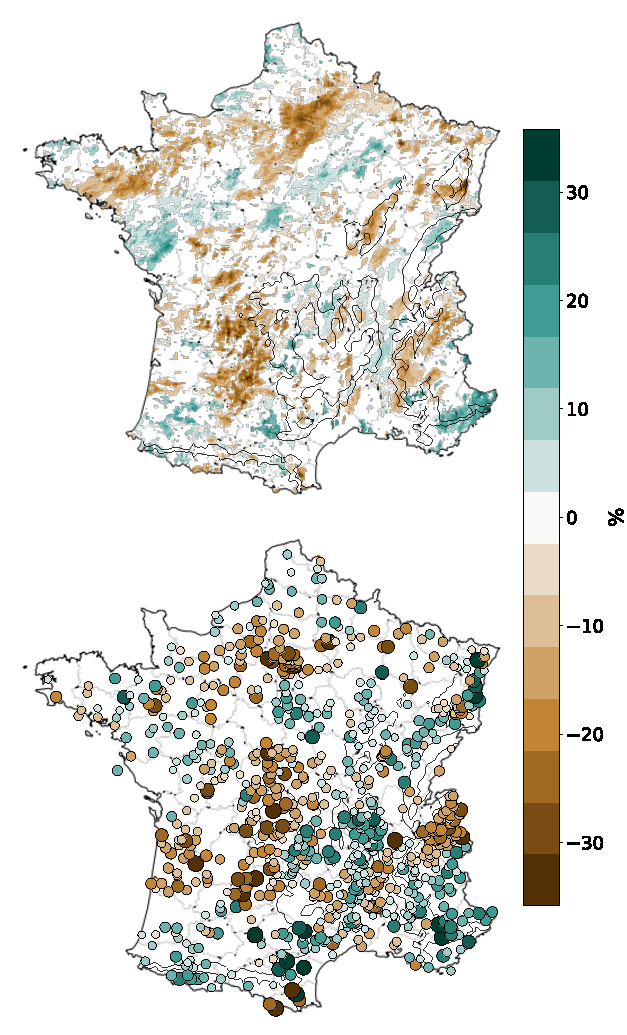
\includegraphics[keepaspectratio]{figures/trend_pluie_son.pdf}}
&
\pandocbounded{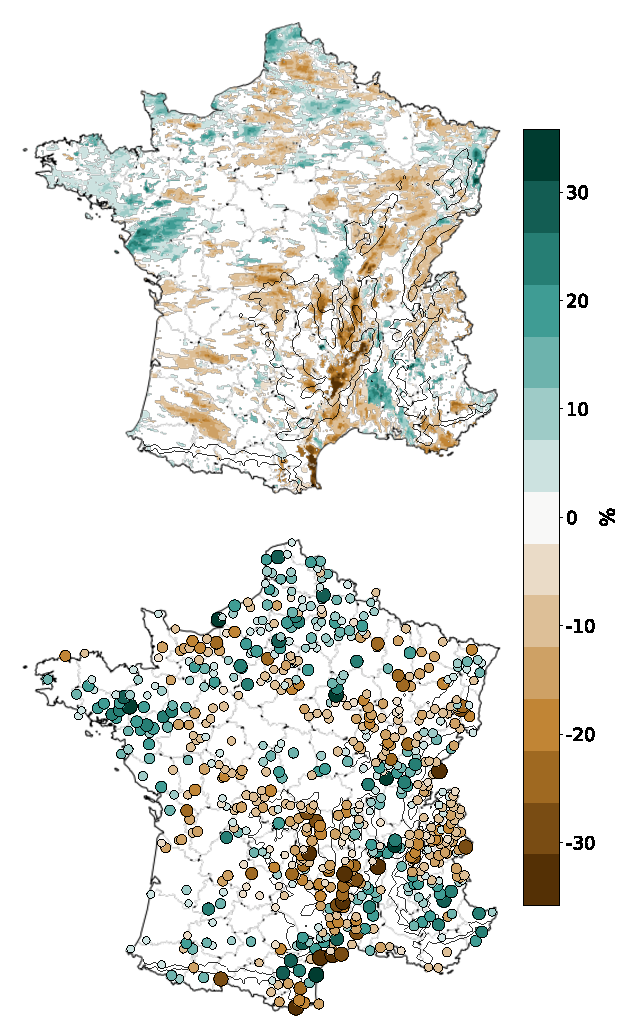
\includegraphics[keepaspectratio]{figures/trend_pluie_djf.pdf}}
&
\pandocbounded{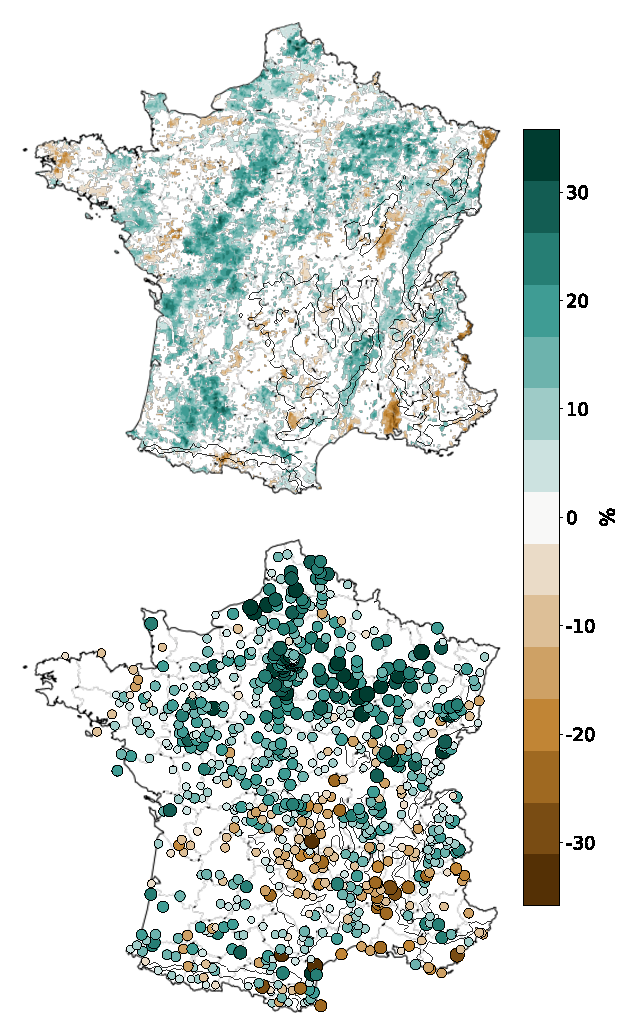
\includegraphics[keepaspectratio]{figures/trend_pluie_mam.pdf}}
&
\pandocbounded{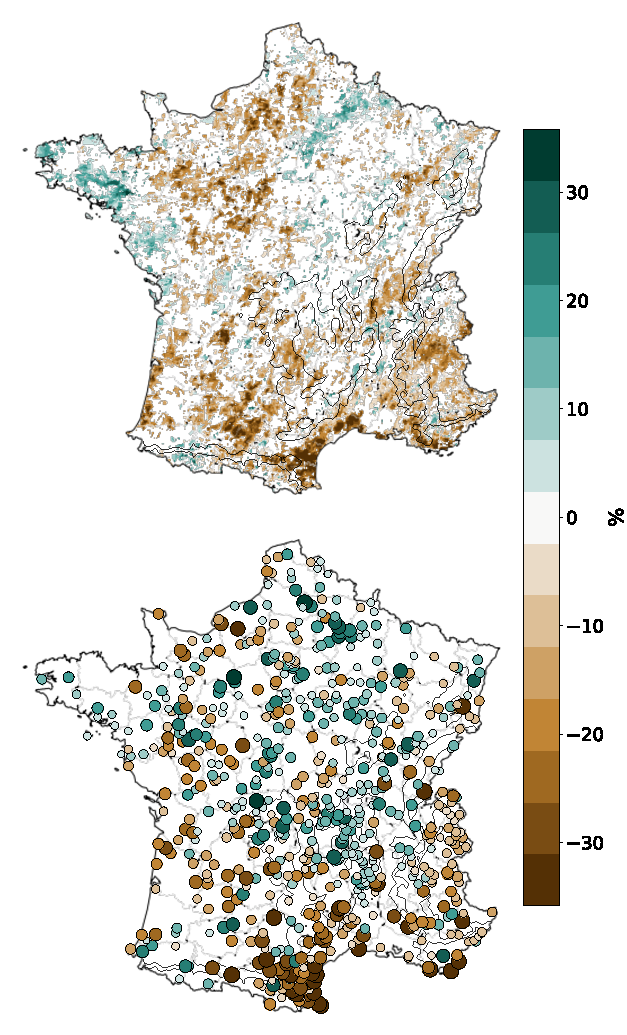
\includegraphics[keepaspectratio]{figures/trend_pluie_jja.pdf}} \\
\small \(r =\) 0.31 (n = 305) & \small \(r =\) 0.39 (n = 353) &
\small \(r =\) 0.19 (n = 344) & \small \(r =\) 0.21 (n = 272) \\
\small \(ME =\) -3.01\% & \small \(ME =\) -2.76\% & \small \(ME =\)
-2.42\% & \small \(ME =\) -5.58\% \\
\end{longtable}

\captionof{figure}{\small Analyse saisonnière (SON, DJF, MAM et JJA) des tendances relatives de 1995 à 2022 (\%) du niveau de retour 10 ans significatif entre le modèle AROME (première ligne) et les stations Météo-France (deuxième ligne) avec la corrélation ($r$), le nombre de stations comparés (n) et le biais ($ME$) issues des maxima de précipitations au pas de temps journalier allant de 1959 à 2022.}

\hfill\break

À l'automne (\textbf{SON}), AROME indique des tendances négatives (−10 à
\textless\,−30\,\%) sur le bassin parisien, le versant occidental du
Massif central et les pré‑Alpes, et une hausse marquée dans le
Mercantour, comme précédemment. Les stations confirment ce schéma, mais
avec une diminution moins prononcée sur les pré‑Alpes et un signal
haussier plus net sur les Alpes du Nord. La vallée du Rhône se distingue
par une augmentation pouvant atteindre localement +40\%. En hiver
(\textbf{DJF}), AROME met en évidence des tendances négatives marquées
--- jusqu'à −40\,\% --- depuis les Pyrénées orientales jusqu'à la haute
crête cévenole ; des diminutions plus modérées (−15\,\%) affectent
également les Alpes du Nord et le Jura. À l'inverse, les façades
atlantique nord et manche présentent des tendances positives de +10 à
+30\%. Les stations confirment ce schéma, tout en étendant la zone de
baisse sur les Alpes du Nord. Au printemps (\textbf{MAM}), le signal est
peu structuré\,: AROME n'isole pas de pattern net, mais suggère des
tendances positives sur la moitié nord et ouest de la France (+15 à
+30\%). Les stations renforcent ce diagnostic, avec une hausse
généralisée sur l'ensemble de la moitié Nord, localement
\textgreater\,+35\%. En été (\textbf{JJA}), AROME met en évidence une
baisse généralisée sur la moitié sud de la France, atteignant −10 à
\textless−30\% le long de l'arc méditerranéen, avec un noyau de
diminution marqué sur les bassins pyrénéens orientaux. Les stations
confirment ce motif spatial.\\

Globalement, AROME reproduit la distribution spatiale des tendances
observées, mais avec une faible corrélation et une extension parfois
réduite --- sur les Alpes du Nord en automne et en hiver, ainsi que sur
la moitié nord de la France au printemps --- et sous‑estime
systématiquement leur amplitude, avec un biais moyen compris entre
−2,42\% (MAM) et −4,87\% (HYDRO).

\paragraph{Données horaires}\label{donnuxe9es-horaires}

Nous passons désormais à l'échelle horaire afin d'évaluer l'éventuelle
intensification des extrêmes infra‑journaliers. Face à l'hétérogénéité
spatiale persistante des tendances saisonnières (Annexes\,2‑4.3.1.2,
HYDRO, SON, DJF, MAM et JJA), nous affinons l'analyse au pas mensuel
(Figure 8).

\begin{longtable}[]{@{}
  >{\centering\arraybackslash}p{(\linewidth - 4\tabcolsep) * \real{0.3333}}
  >{\centering\arraybackslash}p{(\linewidth - 4\tabcolsep) * \real{0.3333}}
  >{\centering\arraybackslash}p{(\linewidth - 4\tabcolsep) * \real{0.3333}}@{}}
\toprule\noalign{}
\begin{minipage}[b]{\linewidth}\centering
\small FEV
\end{minipage} & \begin{minipage}[b]{\linewidth}\centering
\small MAR
\end{minipage} & \begin{minipage}[b]{\linewidth}\centering
\small NOV
\end{minipage} \\
\midrule\noalign{}
\endhead
\bottomrule\noalign{}
\endlastfoot
\pandocbounded{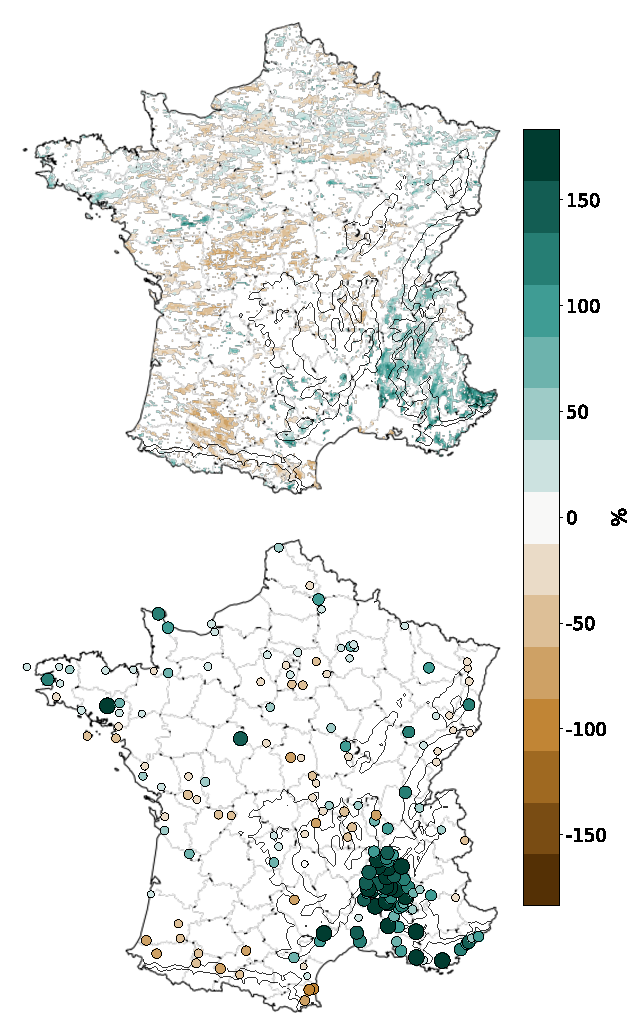
\includegraphics[keepaspectratio]{figures/trend_pluie_fev.pdf}}
&
\pandocbounded{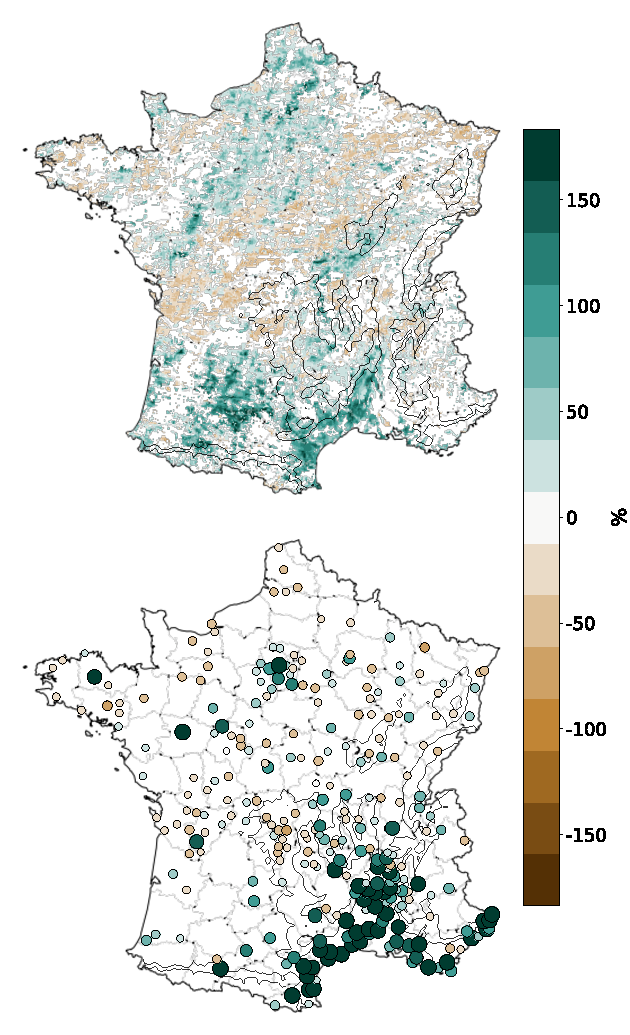
\includegraphics[keepaspectratio]{figures/trend_pluie_mar.pdf}}
&
\pandocbounded{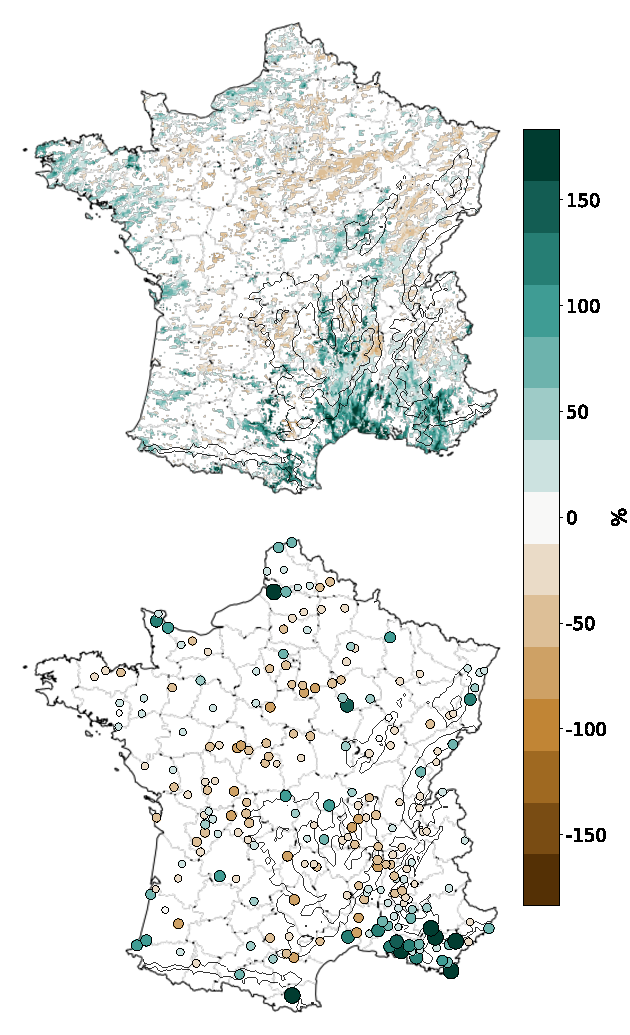
\includegraphics[keepaspectratio]{figures/trend_pluie_nov.pdf}} \\
\small \(r =\) 0.66 (n = 51) & \small \(r =\) 0.48 (n = 136) &
\small \(r =\) 0.24 (n = 72) \\
\small \(ME =\) -56.07\% & \small \(ME =\) -23.33\% & \small \(ME =\)
+8.65\% \\
\end{longtable}

\captionof{figure}{\small Analyse mensuelles (FEV, MAR et NOV) des tendances relatives de 1995 à 2022 (\%) du niveau de retour 10 ans significatif entre le modèle AROME (première ligne) et les stations Météo-France (deuxième ligne) avec la corrélation ($r$), le nombre de stations comparés (n) et le biais ($ME$) issues des maxima de précipitations au pas de temps horaire allant de 1990 à 2022.}

\hfill\break

AROME indique des tendances positives (+25 à \textgreater+150\%) dans la
vallée du Rhône et les pré-Alpes en février (\textbf{FEV}), sur l'arc
méditérannéen ouest (Roussillon--Bas Languedoc) en mars (\textbf{MAR})
et est (bassin azuréen) en novembre (\textbf{NOV}). Les stations
confirment ce schéma, en renforçant nettement le signal sur la vallée du
Rhône en février, avec des tendances environ deux fois plus élevées
qu'AROME. En juin (Annexes 2-4.3.2.2, \textbf{JUI}), AROME et les
stations affichent un signal très majoritairement haussier sur
l'ensemble du territoire, avec des tendances locales pouvant dépasser
+150\%. Cependant, la corrélation spatiale extrêmement faible entre les
deux jeux de données (\emph{r =} 0,07) indique que, si le signe moyen
converge, la localisation des tendances est incohérente/bruitée. Cette
discordance, combinée à la forte variabilité convective estivale et à la
faible longueur des séries mensuelles (1990--2022), appelle à la
prudence.

\subsubsection{Corrélation des tendances relatives entre le modèle AROME
et les stations
Météo-France}\label{corruxe9lation-des-tendances-relatives-entre-le-moduxe8le-arome-et-les-stations-muxe9tuxe9o-france}

Pour objectiver ces divergences et mesurer la robustesse des signaux,
nous examinons désormais les corrélations spatiales entre AROME et les
stations, par saison et mois, afin d'identifier où l'accord est
structurel et où il relève surtout du bruit.\\

À l'échelle quotidienne (1959‑2022), les corrélations des tendances se
situent entre \textbf{0,14} (HYDRO) et \textbf{0,23} (DJF) pour les
saisons et entre \textbf{0,07} (JUI) et \textbf{0,51} (DEC) pour les
mois, plusieurs mois atteignant ou dépassant \textbf{0,40} (JAN, MAR,
AOU, NOV) (Figure 9). Sur la période restreinte (1990‑2022), les valeurs
saisonnières couvrent \textbf{0,13--0,29} et les valeurs mensuelles
\textbf{0,02--0,47} (JAN \textbf{0,47} ; DEC \textbf{0,35}). À l'échelle
horaire (1990‑2022), les saisons présentent des corrélations faibles
comprises entre \textbf{--0,08} (MAM) et \textbf{0,05} (DJF et SON) et
les corrélations suivant les mois s'étendent de \textbf{0,02} (SEP, OCT)
à \textbf{0,42} (FEV).

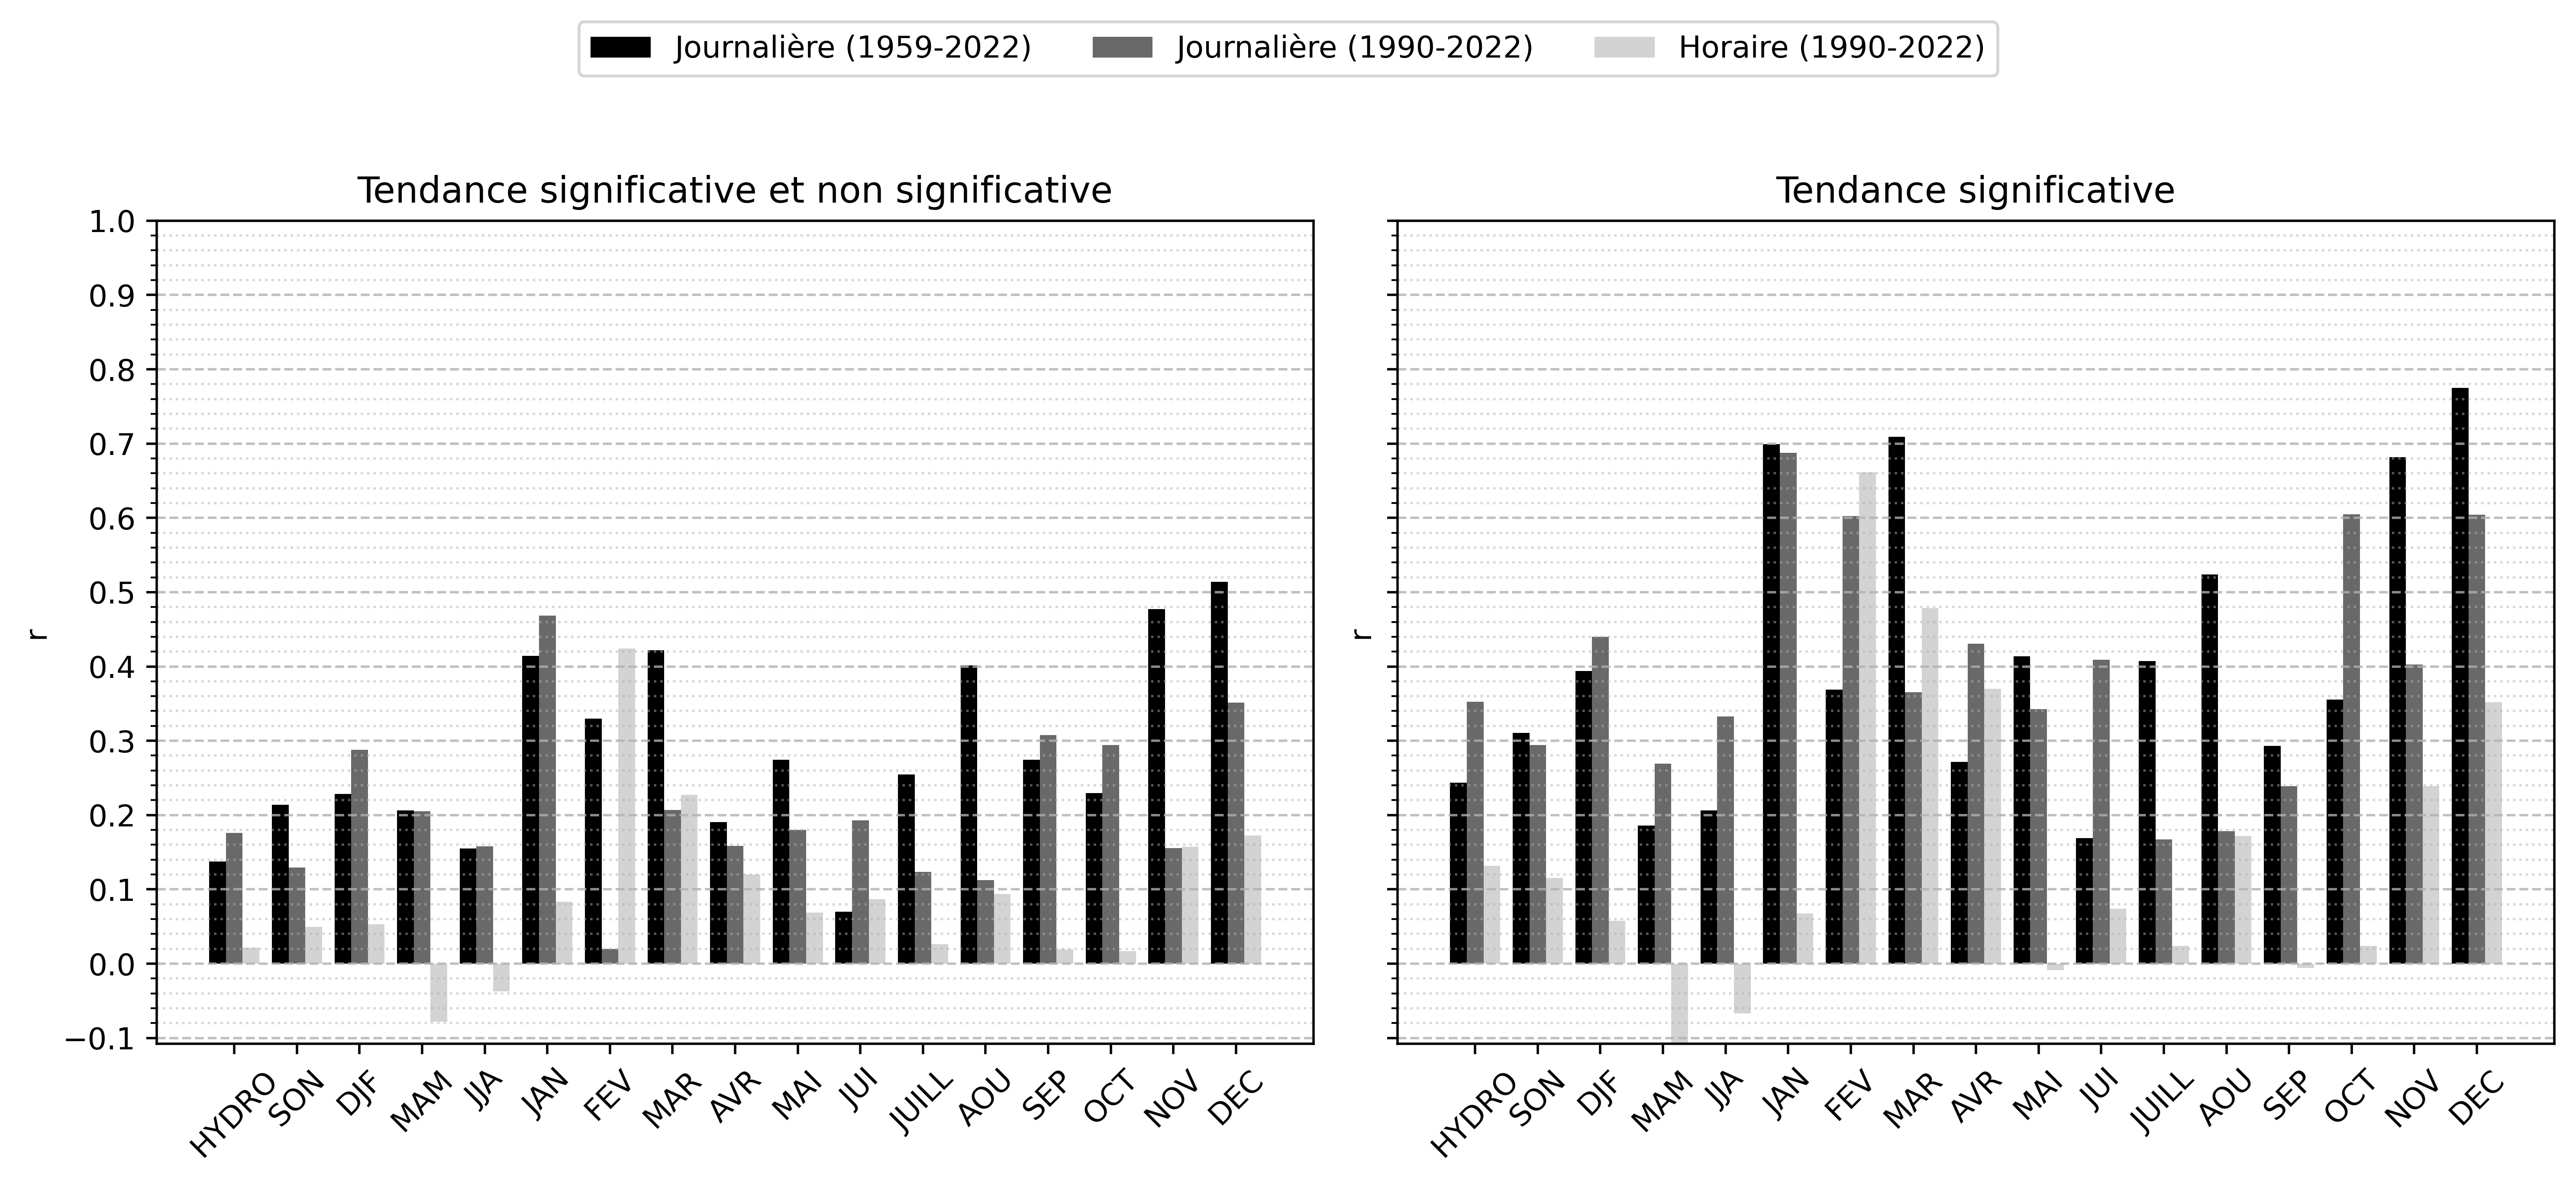
\includegraphics[width=1\linewidth,height=\textheight,keepaspectratio]{figures/histo_z_T_p.png}

\captionof{figure}{\small Corrélations des tendances relatives (toutes et significatives) entre AROME et les stations Météo‑France, par saison et par mois.}

\hfill\break

En restreignant aux tendances significatives par vraisemblance profilée,
l'échelle quotidienne (1959‑2022) affiche des corrélations saisonnières
de \textbf{0,19} (MAM) à \textbf{0,39} (DJF) et des valeurs mensuelles
de \textbf{0,17} (JUI) à \textbf{0,77} (DEC), avec d'autres mois
marquant une corrélation élevée (JAN \textbf{0,70} ; MAR \textbf{0,71} ;
NOV \textbf{0,68} ; AOU \textbf{0,52}). Pour la période restreinte
(1990‑2022), les valeurs saisonnières vont de \textbf{0,27} (MAM) à
\textbf{0,44} (DJF) et les valeurs mensuelles de \textbf{0,17} (JUILL) à
\textbf{0,69} (JAN), avec des valeurs supérieures à 0,60 en février,
octobre et décembre. À l'échelle horaire (1990‑2022), les valeurs
saisonnières couvrent \textbf{--0,20--0,13} et les valeurs mensuelles
\textbf{--0,01--0,66}. La restriction aux tendances significatives
augmente fortement les corrélations quotidiennes, avec des maxima
mensuels élevés. Le gain est marqué en hiver et en fin d'été / automne
(JAN, MAR, NOV, DEC, AOU). À l'échelle horaire, même après filtrage,
l'amélioration reste partielle : quelques mois s'améliorent (FEV) mais
plusieurs périodes sont marquées par des corrélations proches de zéro ou
légèrement négatives (MAI, SEP).

\paragraph{Saisonnalité récurrente de la
performance}\label{saisonnalituxe9-ruxe9currente-de-la-performance}

L'hiver (DJF) et les mois hivernaux isolés (DEC, JAN, MAR) concentrent
les plus fortes corrélations, que ce soit sur la période longue ou
restreinte, et surtout après filtrage. Le printemps (MAM) et le début
d'été (JUI, JUILL) affichent systématiquement les valeurs les plus
basses (ou minima) dans chaque configuration. La fin d'été / automne
(AOU, NOV) fournit des corrélations intermédiaires à élevées une fois
les tendances significatives retenues.

\paragraph{Hiérarchie claire des échelles
temporelles}\label{hiuxe9rarchie-claire-des-uxe9chelles-temporelles}

L'étude journalière est systématiquement plus cohérente spatialement
pour les tendances que l'étude horaire. Le filtrage de significativité
transforme la distribution journalière (multiplication des mois
\textgreater0,60), alors qu'il ne suffit pas à hisser l'horaire à un
niveau comparable (un seul mois \textgreater0,60).

\subsubsection{Distribution des tendances relatives entre le modèle
AROME et les stations
Météo-France}\label{distribution-des-tendances-relatives-entre-le-moduxe8le-arome-et-les-stations-muxe9tuxe9o-france}

Pour compléter l'analyse des corrélations, nous examinons à présent les
boxplots des tendances relatives \emph{significatives} afin d'en
caractériser la distribution (médiane, étendue, valeurs extrêmes) et de
comparer systématiquement AROME aux stations selon les saisons et les
mois.\\

Sur la série journalière 1959--2022 (Fig. 10, panneau \textbf{J}), les
distributions mensuelles des tendances relatives s'étendent de --50\,\%
à +50\,\%, avec quelques extrêmes atteignant ±100\,\% (juillet, août,
décembre). La tendance moyenne est de -4.6\% pour AROME et -1.6\% pour
les stations. Les médianes restent proches de 0 (±10\,\%), mais s'en
écartent positivement au printemps (mars--mai) et négativement en fin
d'hiver ainsi qu'en fin d'été / début d'automne (février, mars, août,
septembre). La forme des distributions est comparable entre AROME et les
stations, bien que l'étalement soit plus marqué pour les stations. Les
médianes sont presque toujours plus élevées pour les stations que pour
AROME.\\

Lorsque l'on restreint la période à 1990--2022 (Fig.\,10, panneau
\textbf{J}*), la dispersion relative augmente pour tous les mois (queues
positives plus longues), tandis que les médianes demeurent modérées
(±20--30\,\%). La moyenne des médianes est de -0,7\% pour AROME et 0,5\%
pour les stations. La tendance moyenne est de 2.4\% pour AROME et 3.5\%
pour les stations. Elles restent positives au printemps (mars--juin) et
en début d'hiver (octobre) (+20 à +50\,\%), et négatives en hiver
(décembre--février), ainsi qu'en août et septembre (--20 à --50\,\%).
Les distributions et leurs médianes sont alors très proches entre AROME
et les stations.\\

Sur les données horaires 1990--2022 (Fig.\,10, panneau \textbf{H}), la
dispersion s'accroît encore avec quelques valeurs extrêmes
\textgreater{} +400\% (tronquées sur la figure). La moyenne des médianes
est de 5,2\% pour AROME et 15,1\% pour les stations. La tendance moyenne
est de 8.5\% pour AROME et 29.1\% pour les stations. Les médianes sont
d'environ ±50\%, ponctuellement jusqu'à ±80/100\%. Elles sont positives
en début d'hiver puis en février et juin (+20 à +60\,\%), et négatives
en août et septembre (--20 à --25\,\%). La distribution est similaire
entre AROME et les stations, mais plus étalée pour ces dernières ; leurs
médianes y dépassent presque toujours celles d'AROME.

\includegraphics[width=1\linewidth,height=\textheight,keepaspectratio]{../outputs/boxplot/violin_signif.pdf}

\captionof{figure}{\small Distribution des tendances relatives significatives entre AROME et les stations Météo‑France, par saison et par mois pour chacune des sources de données (\textbf{J} : données journalières 1959-2022, \textbf{J*} : données journalières 1990-2022, \textbf{H} : données horaires 1990-2022).}

\hfill\break

Quel que soit le type de données (\textbf{J}, \textbf{J}* ou
\textbf{H}), les distributions des tendances relatives s'accordent entre
AROME et les stations en août et septembre. D'un mois à l'autre, les
profils changent sans continuité apparente ; une agrégation purement
saisonnière ne semble donc pas représentative de la variabilité réelle.

\section{Discussion}\label{discussion}

\subsubsection{Fidélité spatiale de la climatologie
simulée}\label{fiduxe9lituxe9-spatiale-de-la-climatologie-simuluxe9e}

Les résultats confirment qu'AROME reproduit correctement les grands
régimes pluviométriques hexagonaux confirmé par la littérature
\citep{Fumiere2020}, \citep{caillaud2021simulation},
\citep{hess-28-2579-2024}, \citep{LucasPicher2024}. Il y a un excédent
orographique sur les Alpes, les Pyrénées et le Massif central, un
gradient atlantique‑continental marqué à l'ouest\,et un déficit
fréquentiel sur le pourtour méditerranéen. Cette cohérence avec la
réalité mesurée témoigne d'une représentation satisfaisante des forçages
dynamiques (transport d'humidité par les flux d'ouest, soulèvement
orographique, circulation de basse couche en Méditerranée).

\subsubsection{Variabilité saisonnière et représentation des
extrêmes}\label{variabilituxe9-saisonniuxe8re-et-repruxe9sentation-des-extruxeames}

La capacité d'AROME à restituer la fréquence et la quantité de
précipitations se maintient tout au long de l'année, mais la performance
chute pour la moyenne des maxima journaliers en été et davantage à
l'échelle horaire. On retrouve le fait qu'AROME sous-estime des
précipitations d'intensité élévées (\textgreater{} 40 mm/h
\citep{Caillaud2021}, \citep{poncet2024convection}) La convection
estivale reste partiellement sous‑résolue malgré la résolution spatiale
de 2,5\,km. Dans cette étude, on a pu montrer (résultats non affichés)
que la corrélation augmente lorsque la fenêtre temporelle s'agrandit à 6
ou 9h. Le modèle pourrait reproduire la cellule orageuse en\,démarrant
trop tard ou trop tôt, en étalant l'intensité sur plusieurs mailles (non
évalué par manque de stations) ou en sous‑estimant les précipitations
maximales. Le pas de 2--3\,km est une étape majeure pour représenter la
convection sans paramétrage, mais il reste trop grossier pour certaines
applications sensibles aux maxima intenses \citep{Prein2015Review}. Il
aurait été intéressant d'introduire les données COMEPHORE (1\,km,
15\,min) de Météo-France dans cette étude mais les réanalyses radar ne
débutent qu'en 1997 avec une qualité médiocre sur les Alpes avant 2007
\citep{Fumiere2020}.

\subsubsection{Tendances des extrêmes de précipitations : cohérences,
divergences et
limites}\label{tendances-des-extruxeames-de-pruxe9cipitations-cohuxe9rences-divergences-et-limites}

\paragraph{Données journalière}\label{donnuxe9es-journaliuxe8re}

La tendance positive et significative sont cohérentes avec l'étude à
l'échelle terrestre de l'\citet{IPCC2021} montrant une hausse du niveau
de retour 10 ans de +6,7\% issu des pluies journalières pour 71\% de la
surface. Les hot-spots sur le Mercantour (+20 à +30\,\%) et, côté
stations, sur la vallée du Rhône (+5 à \textless\,+30\,\%) sont
cohérents avec les travaux montrant une intensification des extrêmes
dans le Sud‑Est de la France et sur les Alpes du Sud de
\citet{blanchet2021explaining}. En automne une augmentation du niveau de
retour 20 ans pourrait atteindre l'ordre de grandeur de sa valeur
moyenne dans le sud‑est alpin. Les tendances haussières marquées des
stations (\textgreater\,+35\%) sur la moitié Nord de la France résonnent
avec les projections françaises qui anticipent des augmentations plus
fortes des extrêmes journaliers dans le Nord sous réchauffement (+20\%
pour +4°C) montré par \citet{soubeyroux:hal-04991790}. Le biais moyen
négatif (−2,4\,\% à −4,9\,\%) signifie que le modèle aplatit
systématiquement les tendances par rapport aux observations, à relier à
la représentation des extrêmes par AROME.

\paragraph{Données horaires}\label{donnuxe9es-horaires-1}

Les signaux sont beaucoup moins robuste au pas de temps horaire qu'au
pas de temps journalier. Ils montrent des tendances très hétérogènes,
souvent peu ou pas significatives, et parfois incohérentes spatialement
entre AROME et les stations (en juin, \emph{r =} 0,07). Cela rejoint le
constat de \citet{IPCC2021} concernant la faible confiance dans une
hausse globale des extrêmes sous‑journaliers, faute de séries longues,
denses et homogènes. Les hausses marquées en février (vallée du Rhône,
pré‑Alpes), mars (arc méditerranéen ouest) et novembre (arc
méditerranéen est) sont compatibles avec les régimes dynamiques et
thermo‑marins propices aux épisodes méditerranéens/transitionnels (fin
d'hiver, intersaison automnale). Le signal doublé par les stations en
février sur la vallée du Rhône souligne le lissages et biais d'amplitude
d'AROME sur les extrêmes horaires. Toutefois, la période restreinte
(1990--2022) offre peu de puissance statistique, et la variabilité
interannuelle convective peut cacher ou mimer une tendance. En juin, la
hausse généralisée (jusqu'à +150\%), mais sans accord spatial entre
AROME et stations montre la variabilité convective locale (orages très
ponctuels) et les erreurs de représentativité point \emph{vs.} maille
deviennent dominantes. C'est un exemple des limites de l'inférence
mensuelle sur les extrêmes convectifs.\\

De nombreuses études régionales mettent en évidence des sensibilités
infra‑journalières de +7 à +14\%/°C, parfois supérieures à
Clausius‑Clapeyron, notamment pour des orages convectifs brefs. L'étude
n'identifie pas de signal clair avec le modèle AROME qui sous‑estime
fortement les pics horaires, alors que les stations captent des pointes
locales. C'est ce à quoi on s'attendait au regard de la part des
tendances des extrêmes liée à Clausius-Clapeyron qui devait
théoriquement être deux fois plus faible que les tendances observées.

\subsubsection{Robustesse statistique des
signaux}\label{robustesse-statistique-des-signaux}

Une fenêtre longue (1959--2022) réduit les incertitudes d'estimation et
échantillonne plusieurs régimes climatiques (phase de global dimming
dominée par les aérosols jusqu'aux années 1980, puis accélération du
réchauffement à partir de la fin des années 1980--1990). Ce mélange de
régimes atténue mécaniquement la pente moyenne\,: une partie du signal
récent est noyée dans la variabilité multidécennale. À l'inverse, une
fenêtre courte (1990--2022) isole le régime dominé par le réchauffement
rapide, la diminution des aérosols sulfatés en Europe et l'accroissement
quasi linéaire du contenu en vapeur d'eau (+7\%/°C), ce qui fait
ressortir des tendances positives plus nettes. Les deux diagnostics sont
donc complémentaires et doivent être interprétés séparément pour ne pas
confondre bruit multidécennal et forçage anthropique de long terme.\\

En première approximation, les distributions mensuelles des tendances
relatives du niveau de retour 10 ans sont centrées sur 0\% sur
1959--2022, tandis que 1990--2022 montre un léger basculement vers des
accroissements, surtout au printemps et en début d'hiver, en phase avec
la littérature sur l'amplification récente des extrêmes journaliers.
Même si des points de rupture ont été autorisés lorsque le LRT le
justifiait, la transition progressive (environ 10\,ans) entre l'ère du
dimming et le régime chaud post‑1985 reste en partie absorbée par les
modèles longue fenêtre, ce qui réduit la pente moyenne par rapport aux
modèles courte fenêtre qui se calent sur la portion quasi linéaire
récente. Ceci éclaire, par exemple, la tendance nationale moyenne
observée de −1,6\% sur 1959--2022 contre +3,5\% sur 1990--2022.\\

Ces différences sont également attendues d'un point de vue statistique :
\citet{DeGaetano2018} montre que, pour des tendances
\textgreater\,0,5\%/an sur le paramètre de localisation \(\mu\), réduire
la fenêtre de 60 à 30\,ans peut modifier la pente estimée des niveaux de
retour décennaux de 10 à 20\,\%. Autrement dit, la longueur de la
fenêtre et la (non)‑stationnarité du climat pèsent fortement sur
l'estimation des tendances, même lorsque des points de rupture détectés
par LRT sont intégrés.

\subsubsection{Signal hivernal, bruit horaire : le filtrage renforce la
cohérence mais AROME peine sur les extrêmes
fins}\label{signal-hivernal-bruit-horaire-le-filtrage-renforce-la-cohuxe9rence-mais-arome-peine-sur-les-extruxeames-fins}

En ne gardant que les tendances significatives on élimine nombre de
sites où le signal est dominé par le bruit climatique, améliorant la
cohérence spatiale des tendances et donc les diagnostics régionaux. À
l'échelle journalière, les valeurs mensuelles des corrélations
AROME--stations oscillent entre 0,40 et\,0,77 après filtrage par
significativité, contre moins de\,0,20 à l'échelle horaire. Ce saut
serait à relier à la difficulté d'AROME à expliquer les maxima
convectifs fins au pas de temps horaire.\\

Le découpage saisonnier met en lumière une hiérarchie marquée par
l'hiver (DJF) qui concentre systématiquement les corrélations les plus
fortes et des hausses modérées à marquées des niveaux de retour. En
hiver, les précipitations en Europe occidentale viennent des
perturbations atlantiques véhiculées par les flux d'ouest. Leur
intensité dépend directement de la quantité de vapeur d'eau dans ces
masses d'air, qui augmente avec la température selon la loi de
Clausius--Clapeyron. C'est pourquoi des hivers plus doux peuvent parfois
être aussi plus pluvieux, même avec une dynamique atmosphérique
identique. Le printemps et le début d'été (MAM--JUI) enregistrent au
contraire les minima de corrélation systématiques. Cela révèle la
difficulté persistante, même à résolution 2,5 km, à représenter
la\,convection faiblement organisée typique de cette saison.\,Le
réchauffement diurne déclenche surtout des orages isolés d'origine
locale. L'influence des perturbations atlantiques diminue, car le
jet‑stream et ses systèmes frontaux se déplacent vers le nord. Le
cisaillement vertical s'affaiblit, empêchant l'organisation des orages
en structures durables. Il en résulte des précipitations brèves, très
localisées et peu structurées que le couple simulation--observations
capture encore mal. En août et septembre, la convergence relative des
distributions (médianes proches et corrélations \textless\,0,20) traduit
une variabilité élevée et une contribution partagée entre épisodes
orageux continentaux et systèmes méditerranéens précoces. La mixité des
mécanismes pluvieux réduit la cohérence entre sites et la capacité
d'AROME à reproduire la saisonnalité des tendances.

\subsubsection{Signaux régionaux : focus sur la vallée du
Rhône}\label{signaux-ruxe9gionaux-focus-sur-la-valluxe9e-du-rhuxf4ne}

La vallée du Rhône semble être un «\,hot‑spot\,» des tendances positives
du niveau de retour, cohérent avec la recrudescence d'événements
cévenols à l'automne et de perturbations orographiques renforcées en
flux de sud \citep{Fresnay2012}. AROME sous‑diagnostique ces hausses
mais en reproduit la localisation, suggérant que la dynamique
(canalisation méridienne et levée orographique) est correctement
simulée, tandis que l'intensité convective demeure sous‑résolue.
\citet{Ribes2019} met en évidence que cette zone\,cumule le plus fort
renforcement observé sur l'ensemble du Midi méditerranéen avec un gain
d'intensité moyen de +22\% des précipitations extrêmes journalières
entre 1961 et 2015. Ils mettent en évidence sur la moitié sud‑est,
incluant Gard, Ardèche et Drôme, un doublement de la fréquence des
évènements\,\textgreater200\,mm en 24h depuis\,1985\,avec la plupart
associés à des pics horaires \textgreater50\,mm.
\citet{blanchet2021explaining} montrent que, depuis les années\,1980,
l'influence méditerranéenne automnale s'est nettement intensifiée et
avancée dans la saison, avec les hausses de niveaux de retour les plus
fortes centrées sur le sillon Rhône‑Alpes et les Cévennes. Ce
«\,hot‑spot\,» est flagrant à l'échelle nationale pour les données
horaires en février. Depuis le début des années\,1990, la température
moyenne des mois d'hiver en France a gagné +0,8°C (différence entre les
normales 1961‑1990 et 1991‑2020 de Météo‑France)\,---\,soit un pouvoir
de rétention d'humidité supplémentaire d'environ +6\% selon la relation
de Clausius‑Clapeyron. Trois leviers pourraient se cumuler en février :
1) la pluie remplace la neige, concentrant la lame d'eau
\citep{ZAQOUT2024131439} ; 2) il existe des pentes de 12\%/°C pour les
extrêmes horaires lorsque T = 0--8°C --- soit presque le double des 7\%
classiques \citep{Drobinski2016} ; et 3) des flux de sud plus humides
injectent davantage de vapeur dans un couloir orographique très efficace
\citep{LorentePlazas2020}.

\section{Conclusion}\label{conclusion}

\section*{Remerciements}\label{remerciements}
\addcontentsline{toc}{section}{Remerciements}

Je tiens à remercier Juliette Blanchet et Antoine Blanc pour
l'encadrement rigoureux, stimulant et bienveillant tout au long de ce
stage. Leurs conseils avisés, leur disponibilité constante et leurs
nombreuses remarques constructives m'ont permis d'approfondir
considérablement mes compétences scientifiques et méthodologiques.

\section*{References}\label{references}
\addcontentsline{toc}{section}{References}

\renewcommand{\bibsection}{}
\bibliography{bibliography.bib}

\newpage

\section*{Annexes 1 : formules
mathématiques}\label{annexes-1-formules-mathuxe9matiques}
\addcontentsline{toc}{section}{Annexes 1 : formules mathématiques}

\subsection*{A.1.1. Obtention de (1)}\label{a.1.1.-obtention-de-1}
\addcontentsline{toc}{subsection}{A.1.1. Obtention de (1)}

Soit la fonction de vraisemblance
\({\displaystyle {\mathcal {L}}(\theta ;x)} : {\displaystyle \theta \mapsto f(x;\theta )}\).
Alors :
\({\displaystyle \log {\mathcal {L}}(\theta ;x_{1},x_{2},\dots ,x_{n})=\sum _{i=1}^{n}\log {\mathcal {L}}(\theta ;x_{i})}\).

Pour \(1 + \xi \frac{x - \mu}{\sigma} > 0\), avec \(\sigma > 0\) :

\[
\begin{aligned}
\log \mathcal{L}(\theta)
&= \sum_{i=1}^n \left[
  -\log \sigma
  - \frac{1 + \xi}{\xi} \log\left(1 + \xi \frac{x_i - \mu}{\sigma} \right)
  - \left(1 + \xi \frac{x_i - \mu}{\sigma} \right)^{-\frac{1}{\xi}}
\right] \\
\log \mathcal{L}(\theta)
&= -n \log \sigma
- \left(1 + \frac{1}{\xi}\right) \sum_{i=1}^n \log\left(1 + \xi \frac{x_i - \mu}{\sigma} \right)
- \sum_{i=1}^n \left(1 + \xi \frac{x_i - \mu}{\sigma} \right)^{-\frac{1}{\xi}}
\end{aligned}
\]

La log-vraisemblance \(\ell(\theta) = \log \mathcal{L}(\theta)\) s'écrit
alors :

\[
\ell(\theta)=
-\sum_{i=1}^n\Bigl[
\log\sigma
+\Bigl(1+\tfrac1{\xi}\Bigr)\log (1+\xi\;\frac{x_i-\mu}{\sigma})
+(1+\xi\;\frac{x_i-\mu}{\sigma})^{-\frac{1}{\xi}}
\Bigr]
\tag{1}
\]

\subsection*{A.1.2. Obtention des
paramètres}\label{a.1.2.-obtention-des-paramuxe8tres}
\addcontentsline{toc}{subsection}{A.1.2. Obtention des paramètres}

\(\mu_1(z_{T,1})\) et \(\sigma_1(z_{T,1})\)

En développant les paramètres soumis à un effet temporel, on a :

\[
\begin{aligned}
\mu_0 + \mu_1 t &= z_{T,0} + z_{T,1} t - \dfrac{\sigma_0 + \sigma_1 t}{\xi_0} \left[ \left( -\log\left(1 - \frac{1}{T} \right) \right)^{-\xi_0} - 1 \right]\\
\mu_0+\mu_1\,t &= \Bigl[\,z_{T,0}
-\dfrac{\sigma_0}{\xi_0}\Bigl(\bigl[-\log(1-\tfrac1T)\bigr]^{-\xi_0}-1\Bigr)
\Bigr]\;+\;\Bigl[\,z_{T,1}-\dfrac{\sigma_1}{\xi_0}\Bigl(\bigl[-\log(1-\tfrac1T)\bigr]^{-\xi_0}-1\Bigr)\Bigr]\,t\\
\end{aligned}
\]

c'est-à-dire, terme à terme :

\[
\begin{aligned}
\mu_0 &\;=\; z_{T,0}
-\dfrac{\sigma_0}{\xi_0}\Bigl(\bigl[-\log(1-\tfrac1T)\bigr]^{-\xi_0}-1\Bigr),\\[0.8em]
\mu_1 &\;=\; z_{T,1}
-\dfrac{\sigma_1}{\xi_0}\Bigl(\bigl[-\log(1-\tfrac1T)\bigr]^{-\xi_0}-1\Bigr).
\end{aligned}
\]





\end{document}
